\documentclass[11pt,a4paper]{article}
\usepackage[UTF8,heading=true]{ctex}
\usepackage[a4paper,left=25mm,right=25mm,top=22mm,bottom=22mm]{geometry}
\usepackage{fontspec,xeCJK,graphicx,booktabs,tabularx,longtable,array,amsmath,amssymb,tikz}
\usetikzlibrary{arrows.meta,positioning}
\usepackage[hidelinks]{hyperref}
\setmainfont{Times New Roman}
\setCJKmainfont{SimSun}[BoldFont=SimHei]
\setCJKsansfont{SimHei}
\setlength{\parindent}{2em}
\setlength{\parskip}{3pt}
\linespread{1.18}
\setlength{\tabcolsep}{5pt}
\setlength{\abovecaptionskip}{5pt}
\emergencystretch=1.5em
\widowpenalty=10000
\clubpenalty=10000
\setcounter{secnumdepth}{3}
\ctexset{section={format=\Large\bfseries},subsection={format=\large\bfseries},subsubsection={format=\normalsize\bfseries}}
\makeatletter
\newcommand{\tableinput}[1]{\@@input #1 }
\newenvironment{inlinefigure}{\par\addvspace{8pt}\noindent\begin{minipage}{\linewidth}\def\@captype{figure}\centering}{\end{minipage}\par\addvspace{8pt}}
\newenvironment{inlinetable}{\par\addvspace{7pt}\noindent\begin{minipage}{\linewidth}\def\@captype{table}\centering\small}{\end{minipage}\par\addvspace{7pt}}
\makeatother
\newcommand{\given}{\,|\,}
\pagestyle{plain}
% Generated only from saved research outputs; units defined in text.
\newcommand{\MainCost}{35126.85}
\newcommand{\MainPurchase}{59482.70}
\newcommand{\MainCharge}{20740.67}
\newcommand{\MainDischarge}{16799.94}
\newcommand{\MainLoss}{3940.73}
\newcommand{\PvCharge}{6247.96}
\newcommand{\RuleCost}{38276.64}
\newcommand{\ReserveCost}{37944.35}
\newcommand{\RulePurchase}{57742.42}
\newcommand{\ReservePurchase}{58060.96}
\newcommand{\RuleSaving}{3149.79}
\newcommand{\ReserveSaving}{2817.50}
\newcommand{\RuleSavingPct}{8.23}
\newcommand{\ReserveSavingPct}{7.43}
\newcommand{\ExtraPurchase}{1740.28}
\newcommand{\EveningState}{5168.13}
\newcommand{\PeakRulePurchase}{715.65}
\newcommand{\LowInitialCost}{35199.30}
\newcommand{\HighInitialCost}{35409.75}
\newcommand{\LowInitialDelta}{72.45}
\newcommand{\HighInitialDelta}{282.90}
\newcommand{\LowInitialPct}{0.21}
\newcommand{\HighInitialPct}{0.81}
\newcommand{\BuyTen}{0.00}
\newcommand{\BuyTwelve}{486.40}
\newcommand{\BuyFourteen}{0.00}
\newcommand{\BuySixteen}{394.93}
\newcommand{\BuyEighteen}{636.98}
\newcommand{\BuyTwenty}{0.00}
\newcommand{\ChargeA}{4500.00}
\newcommand{\DischargeA}{0.00}
\newcommand{\ChargeB}{833.33}
\newcommand{\DischargeB}{5947.42}
\newcommand{\ChargeC}{3954.63}
\newcommand{\DischargeC}{2121.42}
\newcommand{\ChargeD}{6119.37}
\newcommand{\DischargeD}{91.10}
\newcommand{\ChargeE}{0.00}
\newcommand{\DischargeE}{5068.69}
\newcommand{\ChargeF}{5333.33}
\newcommand{\DischargeF}{3571.31}


\begin{document}

\begin{center}
  {\LARGE\bfseries 微网与外部电网电力调控策略}
\end{center}

\section*{摘\quad 要}

本文研究含光伏、储能和外部电网的小区微网购电问题。难点在于光伏与负载随时间变化，电池存在容量、功率和充放电损耗，而普通购电、改单和紧急购电又采用不同的价格规则。为使四问前后连贯，本文先建立统一的十分钟电量流和储能递推关系，再根据各问的信息条件逐步加入供需预测、风险准备、日内预报和波动电价。

针对问题一，建立\textbf{全时段电量流线性规划模型}，统筹光伏直供、外网购电和储能移峰，并用日初、日末储电量相等保证费用比较公平。所得代表日费用为35126.85元，低于峰谷购电策略的38276.64元和光伏空间预留策略的37944.35元。

针对问题二，建立\textbf{周期预测--近期加权准备--跨日线性规划模型}。负载与光伏分别依据历史规律预测，再用近期净需求误差确定安全准备量，以应对五倍价格的紧急购电。2025年2月至12月总费用为13583810.84元，其中普通电费12979560.57元、紧急电费604250.27元；相较等权准备方案节省44.66万元。参数检验表明，0.7的日期衰减在快速适应近期变化和保留足够历史信息之间取得了较好平衡。

针对问题三，建立\textbf{历史融合预报--动态安全准备--日内滚动规划模型}。模型将官方光伏预报与近期历史按过往误差自动融合，并在0:00、6:00、12:00和18:00滚动调整尚未执行的订单。全年总费用为13146535.49元，比不加准备量的初始融合方案节省94.22万元。在日内反馈和改单权限相同的条件下，引入6:00、12:00和18:00的新预报又节省21.78万元，说明后发预报值得使用，但每次是否改单仍需结合调整费和储电状态判断。

针对问题四，将未知波动电价纳入预测和调度。零点一次订电分支采用\textbf{滚动提升树--零点线性规划模型}，总费用为14248570.87元；日内调整分支采用\textbf{滚动岭回归--日内调整线性规划模型}，总费用为13822901.35元。后者虽未取得候选中的绝对最低费用，却以0.016\%的费用差换得更少的紧急购电和更清楚的价格修正依据。逐段回算表明，各方案满足供需平衡、储能容量和充放电功率限制。模型能够在费用、供电风险和解释性之间形成清楚的取舍，可为社区、校园和园区微网的滚动购电提供参考。

\noindent\textbf{关键词：}微网调度；储能优化；滚动规划；风险准备；波动电价

\newpage

\graphicspath{{figures/}}
\section{问题重述}
\subsection{问题背景}
光伏发电能够为小区提供电力，但发电充足的时段与居民集中用电的时段未必一致。与外部电网相连的微网，可以从外网购电补充供给，也可以利用储能设备把电量留到以后使用。当光伏有剩余或外网电价较低时充电，在供电不足或电价较高时放电，是协调本地发电与用电需求的一种方式。

这种调控同时受到供电可靠性与购电成本的约束。提前多买电可能造成浪费，买得太少又可能在实际运行中产生高价补购；电池虽然能缓冲供需变化，却受到储电容量、充放电功率和能量损耗的限制。因此，微网需要根据决策时已经掌握的信息，协调各时段的购电与储能使用，在满足小区负载的前提下尽可能减少费用。

\begin{figure}[htbp]
  \centering
  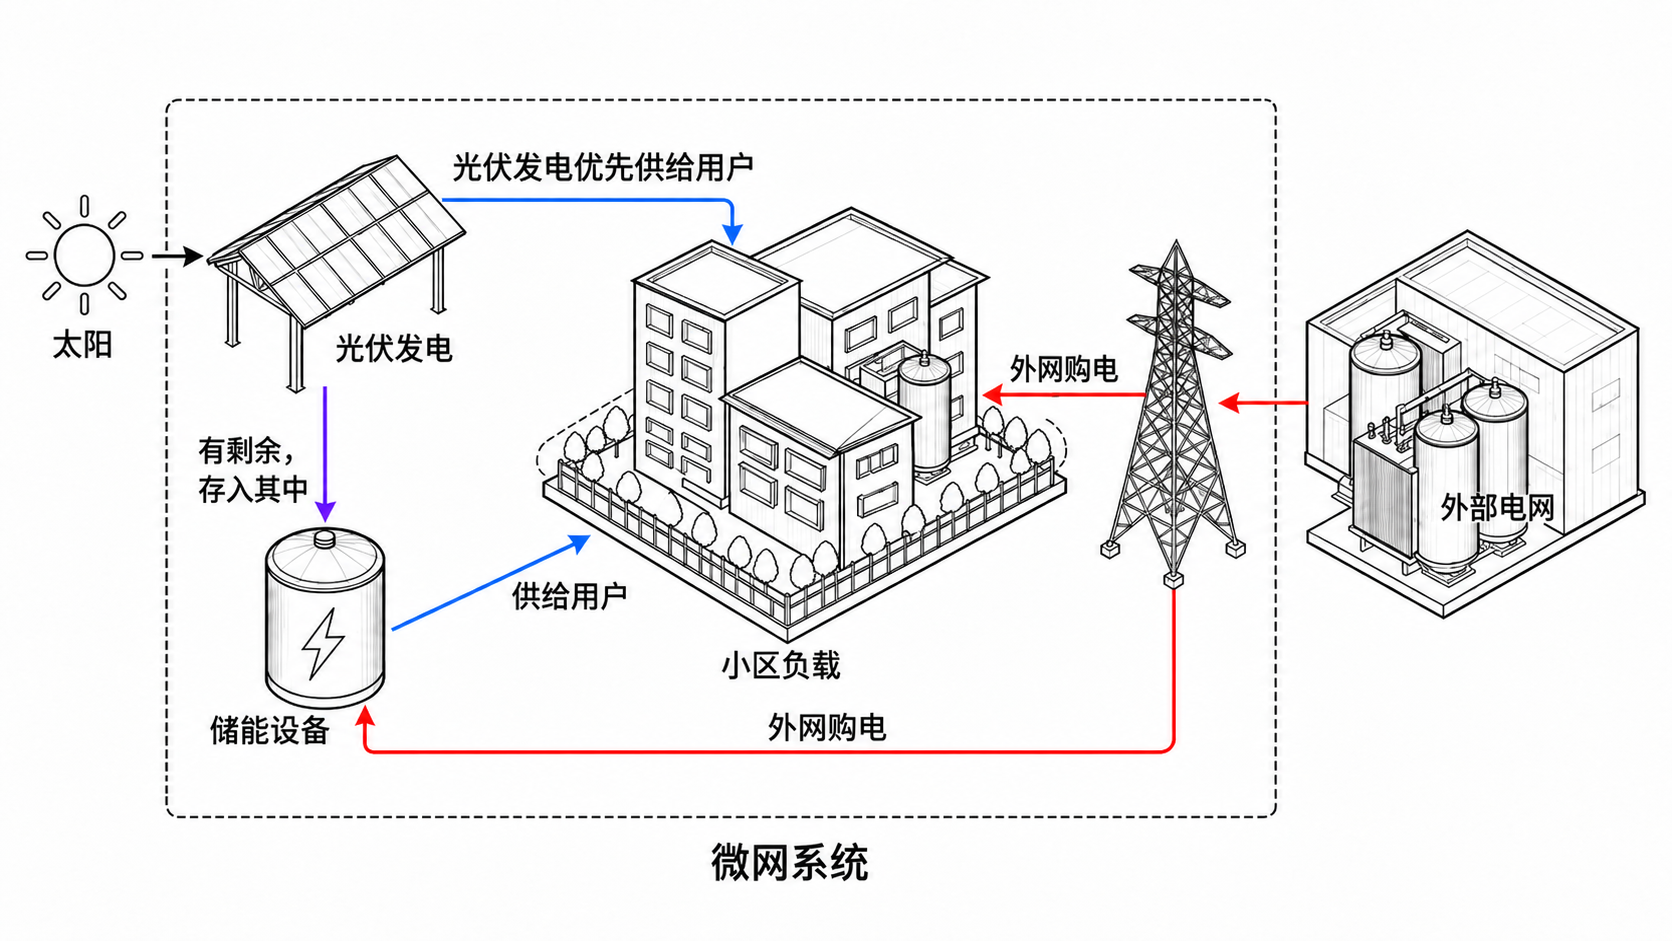
\includegraphics[width=\linewidth,trim=8 8 8 8,clip]{微网系统示意图.png}
  \caption{微网系统的供电关系}
  \label{fig:microgrid-system}
\end{figure}

\subsection{研究对象与共同条件}
研究对象为由光伏、储能设备和外网共同供电的小区微网。附件1给出代表日的电价、负载及光伏预测，附件2给出2025年全年的实际负载和光伏功率，附件3给出每天分四次发布的光伏预报，附件4给出同期波动电价。附件5提供各问的结果文件格式。

储能设备最大容量为12000 kWh，运行储电量须保持在1200--10800 kWh之间，最大充电和放电功率均为5000 kW。题目给定2025年1月1日零点储电量为6000 kWh。功率以kW表示，购电量、充放电量及储电量以kWh表示；各问均须保证微网供电满足小区负载。

\subsection{四问的具体任务}
\textbf{问题一：给定一天供需与电价时的购电安排。}根据附件1和储能参数，在零点安排当天的外网购电及储能充放电，要求当天零点与24点储电量相等。题目中的“每天相同”是指每日重复相同的电价和负载曲线，曲线在一天内仍可随时段变化。需给出满足供电要求、尽可能节省费用的具体安排。

\textbf{问题二：实际供需变化下的每日购电计划。}保持附件1的日内电价，利用附件2所对应的实际运行情景，在每天零点制定当天计划。普通购电按计划量计费；实际运行中供给不足的部分通过紧急购电补足，价格为相应电价的5倍。需同时给出每日计划、实际储能使用及紧急购电情况。

\textbf{问题三：利用更新预报调整购电计划。}在零点取得未来24小时整点光伏预报后制定当天计划，并可在6点、12点和18点取得新预报后调整尚未执行的购电安排。增加的购电量按相应电价的1.5倍收费，减少的部分涉及50\%的违约电价。需给出计划及调整结果，并判断引入日内预报是否值得。

\textbf{问题四：波动电价下的两类购电安排。}使用附件4的电价，分别重新研究问题二和问题三。两条分支分别保留原有的信息条件与调整权限，比较波动电价下的购电、储能使用和费用表现。

\subsection{结果范围与呈现要求}
完整购电结果按10分钟间隔提交。问题一至问题三分别填写\texttt{result1.xlsx}、\texttt{result2.xlsx}和\texttt{result3.xlsx}；问题四的两条分支分别填写\texttt{result4-2.xlsx}和\texttt{result4-3.xlsx}。问题二至问题四的完整结果覆盖2025年2月1日至12月31日，除计划购电和储能记录外，分别保留紧急购电及题目要求的调整记录。

论文按题目指定格式展示重点时段和日期，完整文件保留全部要求的记录。购电展示包括10、12、14、16、18和20点起始的六个10分钟区间，以及全天购电量和费用；储能展示按六个4小时区间分别汇总充电和放电，并列出日初与日末储电量。问题二、三重点展示3月20日、6月21日、9月23日和12月21日，并列出这些日期的紧急购电情况；问题四给出两条分支的相应结果。

\section{问题分析}

\subsection{问题一：已知一天曲线时，电量应当怎样跨时段转移}

问题一给出了完整的日内电价、负载和光伏预测，困难并不在于猜测未来，而在于安排电量何时买、何时存、何时用。光伏最多的时段未必是负载最高的时段，最低电价时段也未必有足够储能空间。若只在低价时尽量充电，电池可能在午间光伏到来前已经装满；若过早放电，又可能在晚间高价和高负载同时出现时失去缓冲能力。因此，需要把全天144个十分钟时段放在一起优化，而不能逐段作出彼此独立的选择。

日初与日末储电量相等是本问的重要条件。它阻止模型通过消耗初始库存制造“今天少买电”的表面低费用，使各方案在相同起点和终点下比较。基于这一结构，问题一采用\textbf{全时段电量流线性规划模型}，将外网直供、外网充电、光伏充电、电池放电和储电量变化统一写入一个优化问题。

\subsection{问题二：计划在零点确定，真实供需随后才出现}

问题二的普通购电必须在每天零点确定，而当天真实负载和光伏还没有发生。附件中的全年数据只能作为事后运行记录和此前历史，不能当作零点已经知道的未来。负载有较明显的星期规律，光伏更受近期天气与季节变化影响，因此二者需要分开预测；预测完成后再合成为净需求，才能保留各自的现实含义。

本问的费用具有明显的不对称性。多订的普通电即使用不完也要付款，少订后真正缺电的部分却要按五倍电价紧急购买。电池能吸收一部分偏差，但会受到最低储电量和放电功率限制，因而“全天总电量够”并不代表每个时段都不会缺电。模型既要给出通常情况下的供需判断，又要依据近期发生过的低估误差留出适量准备。由此采用\textbf{周期预测--近期加权准备--跨日线性规划模型}，并让日末库存自然传给下一天，使当前订电不会把风险简单推迟到次日。

\subsection{问题三：新预报是否值得用，取决于它能否覆盖改单成本}

问题三允许在6:00、12:00和18:00得到新的光伏预报后调整未来订单。新增信息有助于纠正零点判断，但修改订单需要支付调整费，电池也可能已经足以消化预测变化。因此，“获得新预报”和“必须改单”是两件事。合理策略应当先更新未来净需求和实际库存，再比较维持原订单、调增、调减和可能紧急购电的代价。

附件3按小时给出光伏预报，而购电结果按十分钟填写。相邻整点之间采用线性插值，使预报与144个运行时段对应；附件2中的实际光伏只在时段发生后用于更新误差和库存。官方预报反映当天信息，近期同刻历史提供稳定参照，两者各有作用。因而采用\textbf{历史融合预报--动态安全准备--日内滚动规划模型}，并在每个发布时间只调整尚未执行的区间。评价后发预报时，还要把“允许日内反馈和改单”的收益与“新增官方预报”的收益分开，否则会夸大预报本身的贡献。

\subsection{问题四：未来价格也未知后，购电时点本身需要重新判断}

问题四把固定电价改为波动电价。电价变化不只是把原订单重新计价，还会改变什么时候适合充电、什么时候应保留电量以及什么时候放电。因此，需要先用决策时已经发生的价格和历史规律判断未来价格，再把预测价格送入购电与储能规划。

两条分支的权限不同。问题四-2仍在零点一次确定当天普通订单，无法利用当天已发生价格修正，因此更需要表达历史价格、净负荷、星期和季节之间的非线性组合，采用\textbf{滚动提升树--零点线性规划模型}。问题四-3可以在日内更新，价格特征之间相关性较强，又需要解释每次修正来自哪里，因此采用\textbf{滚动岭回归--日内调整线性规划模型}。两种价格模型都只提供决策时的未来判断，最终费用仍按实际电价和真实运行结果结算。


\subsection{四问之间的联系}
四问围绕同一供电系统展开，共享负载满足、光伏利用、储电量变化及设备容量和功率限制。研究首先从问题一的一天安排入手，理清购电与储能转移电量之间的关系；再在问题二中加入实际供需偏差、紧急补购和跨日衔接，使当天计划与实际执行相区分。问题一形成的购电方案仅用于问题二首日启动，后续日期的计划则依据逐日积累的信息制定。

问题三在这一基础上引入按发布时间获得的光伏预报及有代价的计划调整，重点考察提前纠正偏差的作用。问题四分别扩展问题二和问题三，将固定日内电价替换为决策时尚未知晓的波动电价。这样，四问可以共用供电与储能的基本关系，同时分别处理供需偏差、信息更新和价格不确定性；费用比较也可明确对应到普通购电、调整和紧急购电三个来源。


\section{模型假设与符号说明}
\subsection{模型假设}
在题目给定的设备参数和交易规则基础上，作如下运行与信息假设，以明确电量流向、损耗计量及决策时可用的信息。

\textbf{（1）光伏优先直接供给小区负载。}光伏超过负载的部分可用于充电，外网购电既可直接供负载，也可给电池充电；三种电源允许共同供电。光伏优先是本文采用的运行约定。计划电量中能够即时使用或存储的部分予以接收，其余不接收，但普通购电仍按有效计划量结算。最终不能使用或储存的余电不计售电收入，也不对已支付的未利用电量重复计费。

\textbf{（2）采用固定充放电效率与外侧电量计量。}充电效率$\eta_{\mathrm c}$和放电效率$\eta_{\mathrm d}$均取0.90。充电量指进入储能设备前的电量，放电量指设备输出后可供负载使用的电量，5000 kW功率上限也按相应外侧计量。储电状态以电池内部电量表示，计算中不额外引入题目未给出的自放电和寿命折旧项。

\textbf{（3）以10分钟为调度区间。}问题一将附件1的每个采样值作为其后10分钟内的恒定功率和电价，以便将功率转换为时段电量。真实日期中的次日零点按实际日期衔接；问题一使用重复代表日，末尾零点标签映射到本周期开头。

\textbf{（4）储电状态连续衔接。}问题一主方案以6000 kWh开始，并在日末恢复到同一电量；不同起点的影响在本问灵敏度检验中单独考察。问题二至问题四承接前一天的剩余储电量，不逐日重置，也不将问题一的日首尾相等条件直接施加到后续每一天。

\textbf{（5）决策只使用当时可获得的信息。}问题二根据此前已经发生的负载、光伏及当前储电量制定计划，不使用附件3预报；问题三仅使用相应决策时刻已发布的预报。问题四未来实际价格不可提前获知，两条分支分别保留问题二和问题三的调整权限。问题二1月1日缺少更早历史，采用问题一基于附件1得到的购电结构启动，从6000 kWh连续运行，2月初电量由此前运行承接。

\textbf{（6）调整订单以零点原计划为统一结算基准。}对问题三及问题四的调整分支，最终有效普通订单减少部分退回原款，再收取该部分50\%的违约费用；增加部分按1.5倍价格计费，紧急购电另按5倍价格计费。多次修改时旧账冲回，重叠部分不重复收费，采用对应供电时段的价格。调整结果表记最终普通购电总量，零点计划和各次修改分别留存。

\subsection{符号说明}
以$d$表示日期，以$k$表示当天的10分钟区间。第$k$段为$[(k-1)\Delta t,k\Delta t)$，$k=1,\ldots,144$，$\Delta t=1/6$ h。$S_{d,0}$为当天零点储电量，$S_{d,k}$为第$k$段结束时的储电量，一天共对应145个状态边界。问题一只考虑一个代表日，以下模型中省略日期下标$d$。

功率、时段电量和库存分别表示供用电速率、该段累计电量及边界时刻的剩余电量。三者的主要符号与单位列于表\ref{tab:symbols}；决策量的电量流向在问题一模型中进一步说明。

{\small\renewcommand{\arraystretch}{1.18}
\begin{longtable}{>{\centering\arraybackslash}p{3.0cm}>{\raggedright\arraybackslash}p{8.2cm}>{\centering\arraybackslash}p{3.3cm}}
\caption{主要符号及其含义}\label{tab:symbols}\\
\toprule 符号 & 含义 & 单位或取值 \\ \midrule
\endfirsthead
\multicolumn{3}{c}{表\thetable\quad 主要符号及其含义（续）}\\
\toprule 符号 & 含义 & 单位或取值 \\ \midrule
\endhead
\bottomrule\endfoot
$d,\ k$ & 日期下标、日内时段索引 & $k=1,\ldots,144$\\
$\Delta t$ & 一个调度时段的长度 & $1/6$ h\\
$L_{d,k},\ P^{\mathrm{PV}}_{d,k}$ & 小区负载功率、光伏功率 & kW\\
$E^{\mathrm L}_{d,k},\ E^{\mathrm{PV}}_{d,k}$ & 负载电量、光伏电量；由相应功率乘$\Delta t$得到 & kWh\\
$p_{d,k}$ & 对应供电时段的电价 & 元/kWh\\
$m_{d,k}$ & 光伏直接供给负载的电量 & kWh\\
$n_{d,k},\ r_{d,k}$ & 光伏直供后的负载缺口、光伏富余电量 & kWh\\
$x_{d,k}$ & 外网购电中送入储能设备的电量 & kWh\\
$y_{d,k}$ & 送入储能设备的光伏电量 & kWh\\
$z_{d,k}$ & 储能设备输出给负载的电量 & kWh\\
$S_{d,k}$ & 第$k$段结束时的电池内部储电量 & kWh\\
$q_{d,k}$ & 外网购电总量；问题一中由电量分配关系确定 & kWh\\
$E^{\mathrm{ch}}_{d,k},\ E^{\mathrm{dis}}_{d,k}$ & 外侧总充电量$x_{d,k}+y_{d,k}$、总放电量$z_{d,k}$ & kWh\\
$w_{d,k}$ & 未被负载或电池利用的光伏电量 & kWh\\
$S_0$ & 问题一初始储电量，主方案取6000 & kWh\\
$S_{\mathrm{cap}}$ & 设备额定最大容量 & 12000 kWh\\
$S_{\min},\ S_{\max}$ & 允许运行的储电量下限、上限 & 1200、10800 kWh\\
$P_{\max}$ & 外侧充电或放电功率上限 & 5000 kW\\
$\eta_{\mathrm c},\ \eta_{\mathrm d}$ & 充电效率、放电效率 & 均为0.90\\
$C$ & 问题一全天普通购电费用 & 元\\
\end{longtable}}


\graphicspath{{q1_figures/}}
\section{数据预处理与探索性分析}

\subsection{数据预处理}

本文使用题目附件中的代表日供需、全年实际负载与光伏、光伏预报及电价数据。预处理时，统一日期和时间的写法，将同一时刻的负载、光伏和电价对应起来，并保留每次发布的光伏预报。整理后的数值与原表逐项核对一致，没有改变原始数值。以下日均、月均功率按原表日期与采样标签分组取平均；原表末尾的次日零点仍随原标签参与这些描述统计。调度计算则按实际区间建立时间映射，问题一的周期零点单独对应到首段。

经过整理与分析，我们有以下发现。

\subsection{光伏富余与用电需求在时间上错开}

微网面临的首要问题是发电与用电在时间上的不一致。如图\ref{fig:reference}所示，光伏在白天逐渐增强，午间可以覆盖负载并产生富余；傍晚光伏回落后，小区仍有较高的用电需求。电价在晚间也处于较高水平，使这一阶段补充供电的成本更高。图中的负载与光伏功率差直观地反映了这种变化：午间出现富余，傍晚又需要外网或电池补充。

\begin{inlinefigure}
  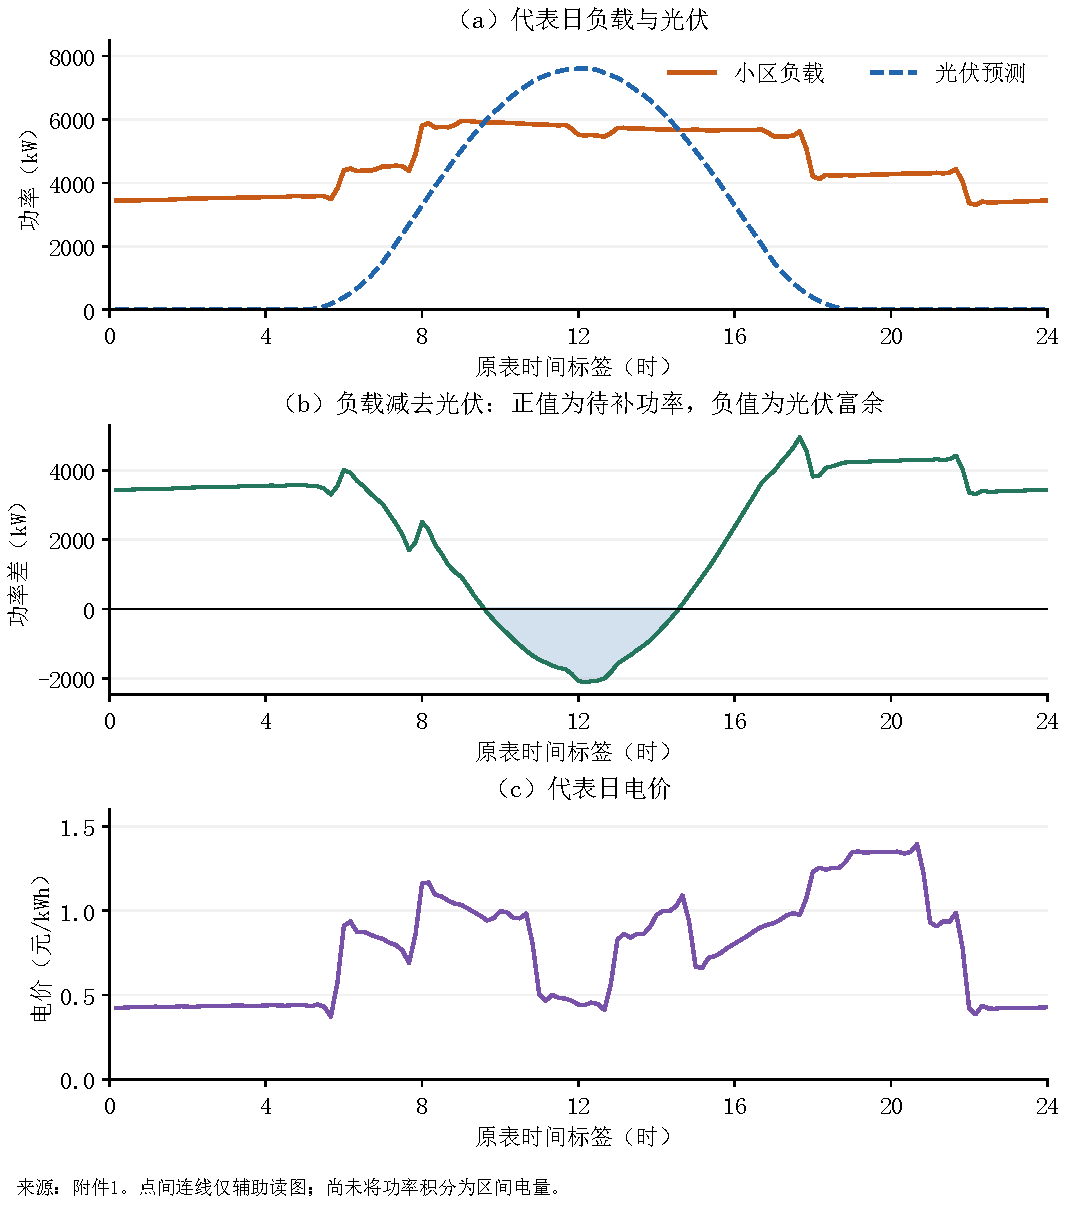
\includegraphics[width=0.82\linewidth]{01_reference_day.pdf}
  \caption{代表日供需与电价的时间错配}
  \label{fig:reference}
\end{inlinefigure}

代表日午间的最大富余功率约为2100 kW，而傍晚需要补充的功率最高接近5000 kW。这说明，白天发电充足并不能直接解决晚间供电问题。电池可以把部分富余电量留到以后使用，但必须先有空间接收，并能在需要时及时放出。因此，购电安排既与当时的供需差额有关，也与之前储存了多少电、之后还要应对多大需求有关。

这种时间错配并非仅出现在代表日：全年有330天出现过光伏超过负载的记录，接收和利用午间富余是经常需要面对的情景。不过，附件1接近全年各时刻的平均供需形状，具体日期仍会出现更高的负载峰值或不同程度的光伏富余。代表日能够说明储能转移电量的基本作用，却不足以代表每一天的运行压力。富余电量最终能利用多少，还取决于当时的电池状态，不能由富余出现的次数直接判断。

\subsection{用电高峰与供需缺口的季节变化不同步}

从图\ref{fig:annual}可以看到，负载与光伏都有明显的年内变化，但二者并不同步。夏季负载较高，同时也有较多光伏补充；进入冬季后，负载虽低于夏季高峰，光伏却明显减少。这使微网对外网补充的需求，不能仅按负载高低来判断。图中的逐日曲线还呈现出月均水平周围的持续起伏，说明季节变化与日际差异同时存在。

\begin{inlinefigure}
  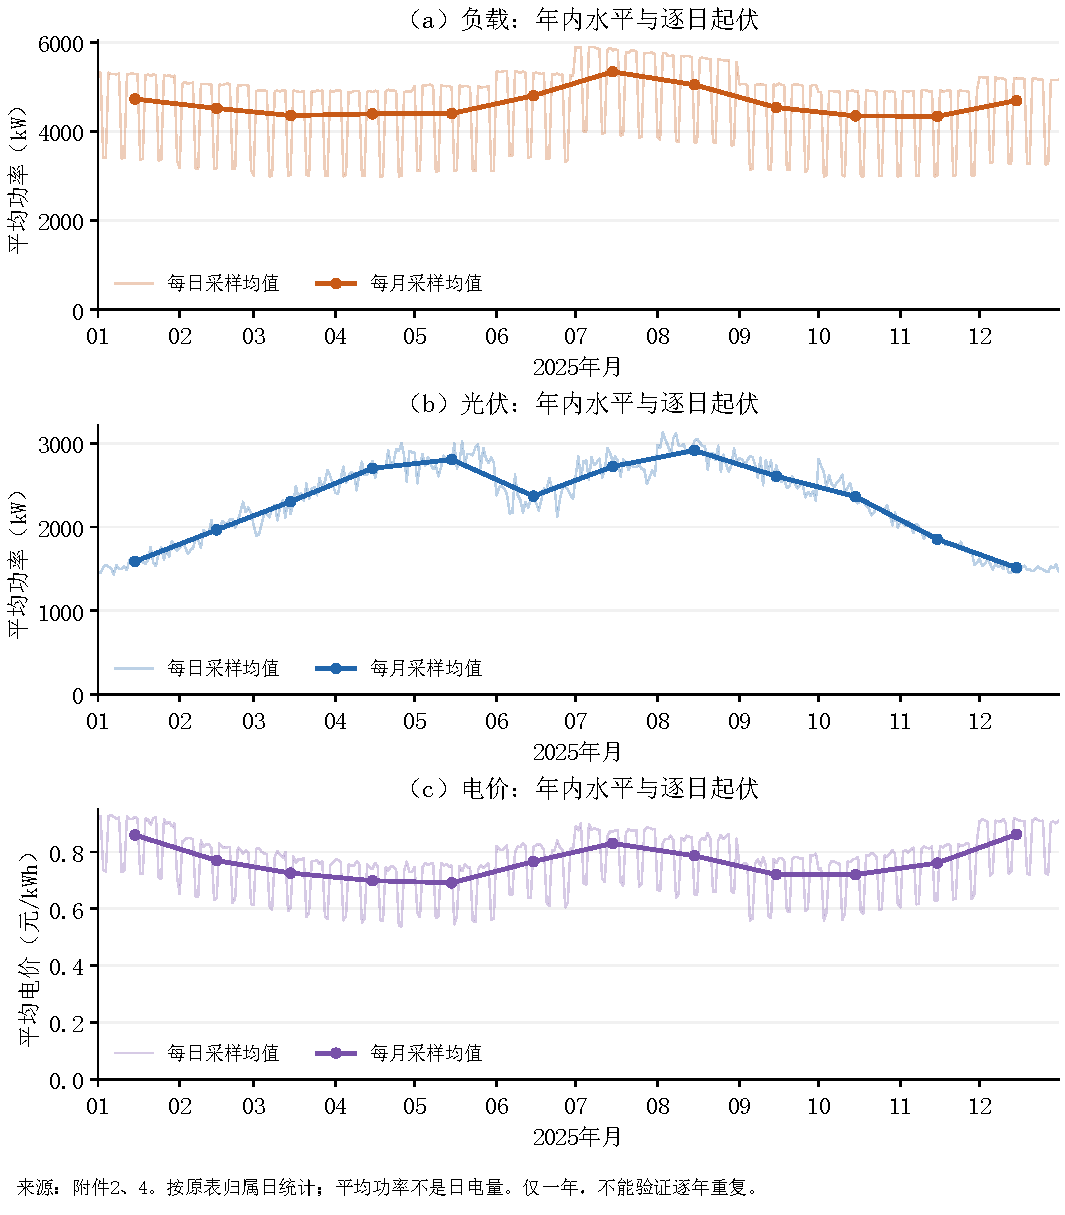
\includegraphics[width=0.82\linewidth]{02_year_and_month.pdf}
  \caption{负载、光伏与电价的年内变化}
  \label{fig:annual}
\end{inlinefigure}

以冬春差异为例，12月平均负载减去光伏后的功率差约为3180 kW，而5月约为1600 kW，前者接近后者的两倍。冬季供需差额较大，并不意味着用电一定更多，而是本地光伏能够承担的部分更少。对储能而言，这也意味着不同季节可供储存的光伏余量和随后需要补充的电力并不相同，全年照用同一套购电、充放电安排，难以适应这种变化。

年内变化也不是平滑的增减。例如，光伏月均功率在6月出现回落，低于相邻月份。附件没有对应天气资料，因此这里只将其视为实际数据中的变化，不推断具体气象原因。现有记录支持2025年存在明显季节差异，是否逐年以同样方式重复，还需要其他年份的数据验证。

\subsection{负载有周重复，电价仍存在跨日波动}

负载除了随季节变化，还表现出清楚的星期差异。按原始日期分组，周五和周六的平均负载比其余五天低约36.8\%，且各月均能观察到这一特点，见图\ref{fig:prices}。这意味着，相邻两天虽然在时间上更近，用电水平却未必更接近；参考历史负载时，同一星期位置的记录也可能提供有用信息。该分组来自附件日期，不据此推断居民的具体作息制度。

\begin{inlinefigure}
  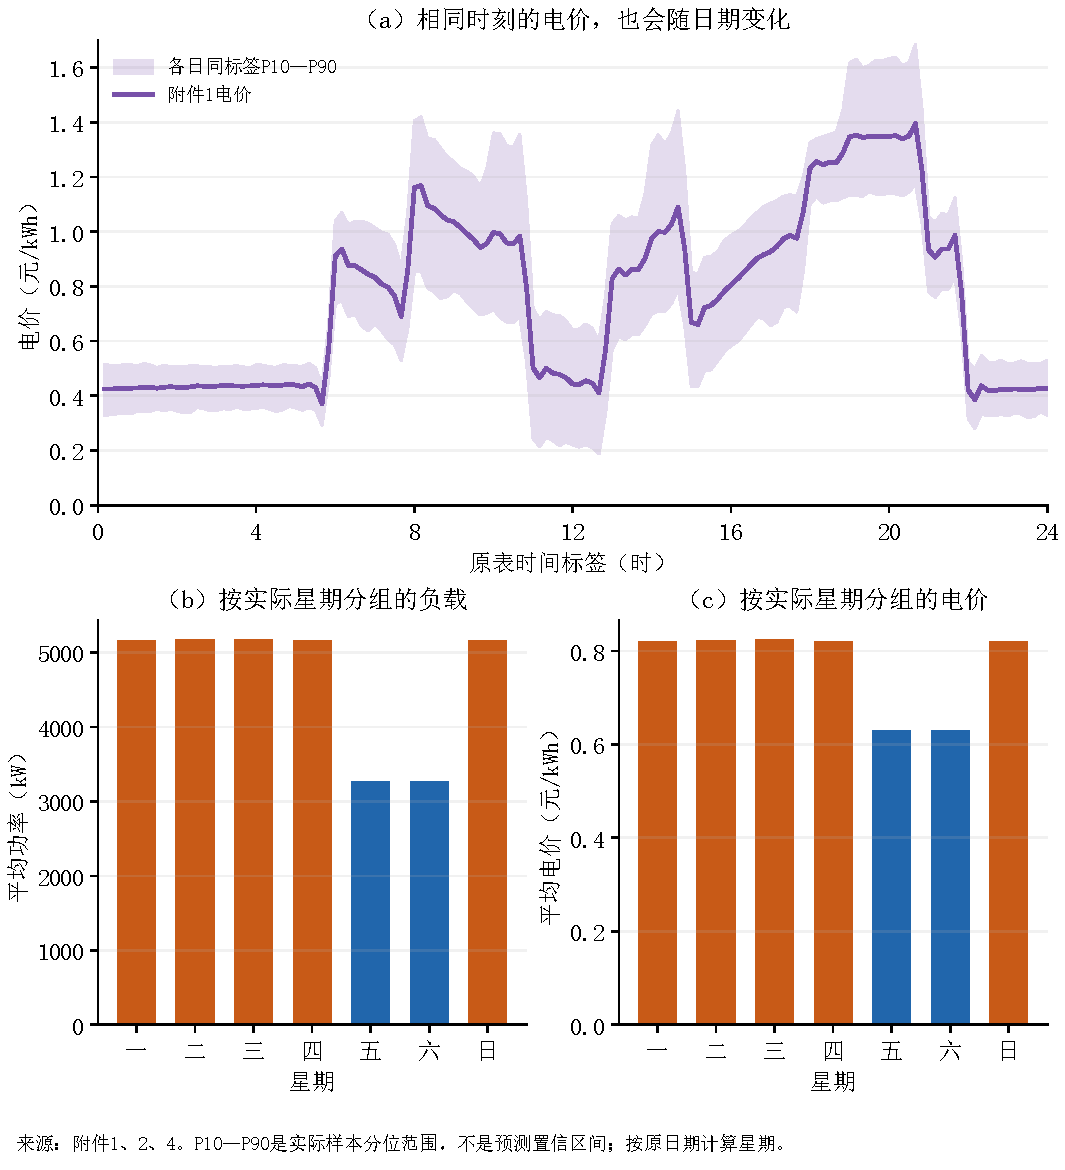
\includegraphics[width=0.78\linewidth]{06_prices_and_weekdays.pdf}
  \caption{不同星期的用电差异与同一时刻的电价波动}
  \label{fig:prices}
\end{inlinefigure}

将序列与一周前的数值比较，并扣除各月相同时刻的平均轮廓后，负载和电价仍保持较强的相关性，而光伏的一周相关性已接近零。光伏原先较高的相似程度，主要来自白天发电、夜间接近零的共同形状。因此，这几类数据不能仅因都呈现重复起伏，就被视为具有相同的周规律；历史信息的参考方式需要适应各自的变化特点。

电价还存在同一时刻、不同日期之间的差异。图\ref{fig:prices}中的阴影给出全年各日同一时刻价格的第10至第90百分位范围，其宽度反映出固定日内曲线没有呈现的波动。历史上较便宜的时段仍可作为参考，但并不保证下一天也同样便宜。按第四问采用的信息条件，未来真实价格尚不可知，提前充电的收益也就存在不确定性：低价购电能否弥补充放电损耗，取决于之后实际遇到的价格和用电需求。

\subsection{光伏预报更新的改善与局限}

附件3的预报整体呈现出提前越久、误差越大的特点，如图\ref{fig:forecast}所示。比较时，将预报与同一目标整点的实测值对应，以两者绝对差的平均值衡量偏差；年末超出实测覆盖范围的36条预报不参与误差计算。图中还区分了全部记录与实际有光伏的记录：夜间接近零的数值会降低总体平均误差，因此仅看总体结果，容易忽略实际发电时更大的供需偏差。

\begin{inlinefigure}
  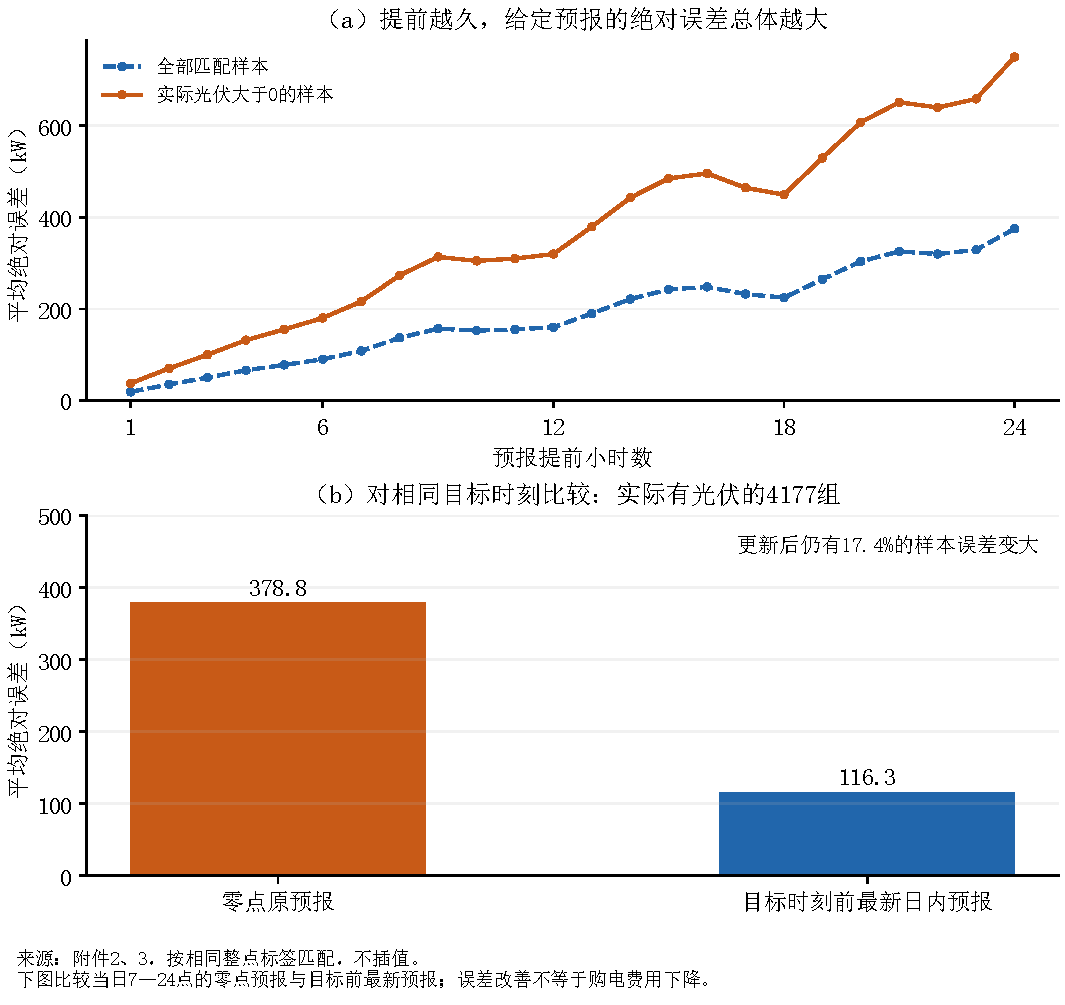
\includegraphics[width=0.78\linewidth]{07_forecast_accuracy.pdf}
  \caption{预报提前量与日内更新对光伏预报误差的影响}
  \label{fig:forecast}
\end{inlinefigure}

为直接观察更新的作用，对每天7点至24点的同一目标时刻，比较零点预报与目标发生前已经发布的最新预报。在实测光伏大于零的4177组配对中，平均绝对误差由约379 kW降至116 kW，减少约69\%。这说明，日内更新确实改善了这组数据中对未来光伏的判断。不过，仍有约17.4\%的配对在更新后误差增大，新预报并非每次都更准确。这里按实测值分组是为了观察发电时的误差，制定计划时并不能提前知道实际光伏。

更准确的信息为调整购电提供了依据，但其经济作用还取决于电池和合同。如果原计划的偏差可以由电池吸收，修改购电量未必划算；如果预计偏差较大、储能又缺少调节余地，提前调整才可能减少昂贵的紧急补购。预报更新的价值取决于它是否改变了实际需要的购电量，以及节省的补购费用能否抵偿调整费用，不能直接用平均误差的降幅代表节费比例。

\section{问题一的模型建立与求解}
\subsection{求解思路与模型选择}

\textbf{全时段电量流线性规划模型。}

附件1给出了同一天内的供需和电价曲线，问题一的关键在于把有限的储能用在合适的时段。若仅在电价低时充电、电价高时放电，可能过早占满午间所需的储能空间，也可能在真正的价格高峰到来前用完可放电量。因此，本文以各时段的电量分配为决策对象，将全天购电和储能变化联系起来，并与两种直观的峰谷购电策略比较，以确定问题一采用的方案。

\subsubsection{时段划分与决策变量}
将一天分为144个10分钟区间，使用第$k$段起点的采样值代表该段内的功率。相应的负载电量与光伏电量为
\begin{equation}
 E^{\mathrm L}_k=L_k\Delta t,\qquad E^{\mathrm{PV}}_k=P^{\mathrm{PV}}_k\Delta t,
 \qquad \Delta t=\frac{1}{6}\ \mathrm h.
 \label{eq:energy_conversion}
\end{equation}
例如，某段负载功率为6000 kW，该10分钟所需电量为1000 kWh。输入表中的零点虽排在末尾，但在重复代表日内对应第一段00:00--00:10；其余记录按实际时刻对应区间，而不直接以行号表示时间。

按光伏优先直接供负载的假设，先计算直供电量$m_k$、剩余负载缺口$n_k$和光伏富余$r_k$：
\begin{equation}
 \begin{aligned}
 m_k&=\min\{E^{\mathrm L}_k,E^{\mathrm{PV}}_k\},\\
 n_k&=E^{\mathrm L}_k-m_k,\qquad r_k=E^{\mathrm{PV}}_k-m_k.
 \end{aligned}
 \label{eq:pv_first}
\end{equation}
这三项均由已知数据确定。它们将同一时段分为负载需要补电或光伏存在富余两种情形，避免将本可直接使用的光伏先送入电池而产生不必要的损耗。

每段设置四个连续决策量：外网用于充电的电量$x_k$、光伏用于充电的电量$y_k$、电池向负载输出的电量$z_k$，以及段末内部储电量$S_k$。四者均以kWh计量，但前三者按设备外侧计量，$S_k$按电池内部计量。为说明购电量与这些变量的关系，将电量流向整理为图\ref{fig:energy_paths}。

\begin{inlinefigure}
 % Q1 energy-path definition: report 12.2, 15; external-side kWh.
\begin{tikzpicture}[>=Stealth, node distance=16mm, every node/.style={font=\small},
  box/.style={draw=black,rounded corners=2pt,minimum width=23mm,minimum height=10mm,align=center},
  lab/.style={fill=white,inner sep=2pt}]
\node[box] (grid) at (0,1.25) {外部电网};
\node[box] (pv) at (0,-1.25) {光伏发电};
\node[box] (battery) at (5,0) {储能设备\\$S_{k-1}\longrightarrow S_k$};
\node[box] (load) at (10,1.25) {小区负载};
\node[box] (waste) at (10,-1.25) {未利用光伏};
\draw[->] (grid.east) -- node[lab,above] {$n_k-z_k$} (load.west);
\draw[->] (grid.south east) -- node[lab,above,sloped] {$x_k$} (battery.north west);
\draw[->] (pv.north east) -- node[lab,above,sloped] {$y_k$} (battery.south west);
\draw[->] (battery.north east) -- node[lab,below,sloped] {$z_k$} (load.south west);
\draw[->] (pv.south) -- (0,-2.65) -- node[lab,below] {$m_k$：光伏直供} (11.9,-2.65) -- (11.9,1.25) -- (load.east);
\draw[->] (pv.east) -- node[lab,pos=.70,above] {$w_k=r_k-y_k$} (waste.west);
\end{tikzpicture}

 \caption{问题一的电量分配关系（各箭头表示该时段的电量）}
 \label{fig:energy_paths}
\end{inlinefigure}

图中，外网既补足电池放电后的负载缺口，也可为以后使用而充电，因此总购电量为
\begin{equation}
 q_k=n_k-z_k+x_k. \label{eq:purchase}
\end{equation}
总充电量为$E^{\mathrm{ch}}_k=x_k+y_k$，总放电量为$E^{\mathrm{dis}}_k=z_k$；未利用光伏为$w_k=r_k-y_k$。这样，购电量不再需要作为独立变量，供电和储能的每一条去向仍可单独核对。

\subsubsection{目标函数}
问题一只计普通外网购电费用。光伏为小区提供本地电源，储能损耗通过额外所需的购电量反映，不另加一笔损耗费用；题目也未给出售电收入或电池寿命成本。因此，以全天购电费用最小为目标：
\begin{equation}
 \min C=\sum_{k=1}^{144}p_kq_k
       =\sum_{k=1}^{144}p_k(n_k-z_k+x_k).
 \label{eq:objective}
\end{equation}
这里$p_k$的单位是元/kWh，$q_k$已经是10分钟电量，计算费用时不再乘$\Delta t$。目标最小化的是费用，而非购电总量；适度增加低价购电，即使带来充放电损耗，也可能减少更昂贵时段的购电支出。

\subsubsection{约束条件}
\textbf{（1）供电与光伏分配。}各时段的负载均需得到满足，充入电池的光伏不能超过该段富余，电池放电不能超过直供后的缺口：
\begin{equation}
 \begin{gathered}
 x_k\geq0,\qquad 0\leq y_k\leq r_k,\qquad 0\leq z_k\leq n_k,\\
 m_k+(q_k-x_k)+z_k=E^{\mathrm L}_k,\qquad
 m_k+y_k+w_k=E^{\mathrm{PV}}_k,\quad w_k\geq0.
 \end{gathered}
 \label{eq:balance}
\end{equation}
其中两条等式由式\eqref{eq:pv_first}和式\eqref{eq:purchase}直接保证。$q_k-x_k=n_k-z_k$为外网直接供负载的电量；允许富余光伏无法全部存入，但不给未利用电量附加售电收益。

\textbf{（2）充放电功率。}容量表示能存多少，功率表示每段能充入或放出多快。最大充电功率和放电功率均为5000 kW，故
\begin{equation}
 x_k+y_k\leq P_{\max}\Delta t,\qquad z_k\leq P_{\max}\Delta t,
 \qquad P_{\max}=5000\ \mathrm{kW}.
 \label{eq:power}
\end{equation}
每段外侧充电量或放电量因此不超过833.33 kWh。此上限约束储能设备，外网直接向负载供电的部分不占用电池充放电功率。

\textbf{（3）储电量变化及运行区间。}充电损耗发生在电量进入电池时，放电损耗发生在电量输出时，故
\begin{equation}
 S_k=S_{k-1}+\eta_{\mathrm c}(x_k+y_k)-\frac{z_k}{\eta_{\mathrm d}},
 \qquad \eta_{\mathrm c}=\eta_{\mathrm d}=0.90,
 \label{eq:soc}
\end{equation}
\begin{equation}
 1200\leq S_k\leq10800,\qquad k=1,\ldots,144.
 \label{eq:soc_bound}
\end{equation}
向设备输入100 kWh只能使内部库存增加90 kWh，而向负载输出90 kWh需要从内部扣除100 kWh。因此，外部电量经过一次完整充放后，能够用于负载的比例为$0.9\times0.9=0.81$。设备达到1200 kWh下限即不能继续放电，并不需要等到电量降至零。

\textbf{（4）日首尾电量相等。}主方案取日初储电量6000 kWh，并要求
\begin{equation}
 S_0=S_{144}=6000\ \mathrm{kWh}.
 \label{eq:cyclic}
\end{equation}
将式\eqref{eq:soc}对全天求和可得
\begin{equation}
 \sum_{k=1}^{144}z_k=\eta_{\mathrm c}\eta_{\mathrm d}
 \sum_{k=1}^{144}(x_k+y_k)=0.81\sum_{k=1}^{144}(x_k+y_k).
 \label{eq:daily_energy}
\end{equation}
这说明当天输出的储能电量需要由当天充电补回，不能依靠消耗初始库存制造低费用。6000 kWh确定主方案的比较条件，日内储电量仍可在允许区间内变化。

\subsubsection{线性结构与求解方法}
上述目标与约束均为线性关系。式\eqref{eq:pv_first}虽然含有最小值运算，但作用于已知供需数据，并未引入非线性决策。每段四个变量，共576个连续变量，144条储电递推等式将全天安排联系起来。

还需说明为何没有额外设置充电、放电的二元开关。在本问正电价、外网可直接供负载的条件下，同时充放电只会增加损耗。若某段$x_k>0$且$z_k>0$，则$n_k>0$、$r_k=0$，因而$y_k=0$。令$\delta=\min\{x_k,z_k/0.81\}>0$，将$x_k$减少$\delta$，同时将$z_k$减少$0.81\delta$，则
\begin{equation}
 \Delta S_k=-0.9\delta+\frac{0.81\delta}{0.9}=0,
 \qquad \Delta q_k=-0.19\delta<0.
 \label{eq:no_cycle}
\end{equation}
这一调整不改变储电轨迹，不破坏功率或供电约束，却严格降低费用，故同时充放不可能是最优选择。因此，本问可直接采用连续线性规划；若出现负电价或新增离散开关限制，这一结论需重新检验。

求解时，先按时间映射生成144段电量与价格，再将式\eqref{eq:objective}和式\eqref{eq:balance}--\eqref{eq:cyclic}整理成线性规划的系数矩阵与变量上下界，使用SciPy的\texttt{linprog}接口调用HiGHS。求解器以最优状态正常终止，并输出逐段购电、充放电与储电量。数值最优性及逐段约束另作独立复核，结果见本问检验部分。

\subsubsection{模型比较与方案选择}
为判断全天统一安排的实际收益，设置两种具有直观含义的参照策略。峰谷电价策略根据低价、高价门槛及目标储电量安排充放电，并考虑充放电损耗；光伏空间预留策略在相同规则上，进一步根据后续富余光伏限制提前充电，避免过早占满电池。线性规划则不预设价格门槛，而是在同一供需与设备条件下，同时确定所有时段的安排。

比较统一使用附件1的代表日、充放各90\%的效率及首尾6000 kWh条件。两种规则分别考察27组相同的参数组合：低价门槛取电价的15\%、25\%、35\%分位，高价门槛取65\%、75\%、85\%分位，目标储电量取6000、8400、10800 kWh。两者均按剩余时段的充放能力保护日末目标，恢复库存所需的实际购电全部计费，再分别取所考察组合中费用最低的结果。

峰谷电价策略、光伏空间预留策略与线性规划的全天费用依次为\RuleCost{}元、\ReserveCost{}元和\MainCost{}元。线性规划相较前两者分别节省\RuleSaving{}元和\ReserveSaving{}元，降幅为\RuleSavingPct{}\%和\ReserveSavingPct{}\%，且三种入选安排均满足逐段约束、没有未利用光伏。由此，本文选择线性规划作为问题一的购电与储能调度方案。它的优势既有实际费用比较的支持，也有在所列约束下统筹全天电量的结构依据。

光伏预留本身的作用并非在所有参数下都相同。在27组相同参数的配对中，18组费用降低、9组相同；尤其在峰谷策略费用最低的那组参数下，加入光伏预留并未改变结果。因此，预留策略各自调参后的费用较低，不能全部归因于新增预留机制。上述比较限于给定代表日和已考察的规则参数，不将规则的局部搜索结果称为该类方法的全局最优，也不据此评价未实际运行的其他算法。

\subsubsection{购电安排与结果分析}
主方案全天购电\MainPurchase{} kWh，费用\MainCost{}元，储能外侧累计充电\MainCharge{} kWh、累计放电\MainDischarge{} kWh。题目指定的六个购电区间及4小时储能汇总分别列于表\ref{tab:purchase}和表\ref{tab:storage}，其余10分钟购电结果保存在\texttt{result1.xlsx}中。

\begin{inlinetable}
 \caption{问题一指定区间的购电量及全天费用}\label{tab:purchase}
 \renewcommand{\arraystretch}{1.23}
 \begin{tabularx}{\linewidth}{l*{3}{>{\centering\arraybackslash}X}}
 \toprule
 时间段 & 10:00--10:10 & 12:00--12:10 & 14:00--14:10\\
 购电量/kWh & \BuyTen & \BuyTwelve & \BuyFourteen\\ \midrule
 时间段 & 16:00--16:10 & 18:00--18:10 & 20:00--20:10\\
 购电量/kWh & \BuySixteen & \BuyEighteen & \BuyTwenty\\ \midrule
 全天购电量/kWh & \multicolumn{3}{c}{\MainPurchase}\\
 全天购电费/元 & \multicolumn{3}{c}{\MainCost}\\
 \bottomrule
 \end{tabularx}
\end{inlinetable}

\begin{inlinetable}
 \caption{问题一各4小时区间的储能充放电量}\label{tab:storage}
 \renewcommand{\arraystretch}{1.23}
 \begin{tabularx}{\linewidth}{l*{3}{>{\centering\arraybackslash}X}}
 \toprule
 时间段 & 00:00--04:00 & 04:00--08:00 & 08:00--12:00\\
 充电量/kWh & \ChargeA & \ChargeB & \ChargeC\\
 放电量/kWh & \DischargeA & \DischargeB & \DischargeC\\ \midrule
 时间段 & 12:00--16:00 & 16:00--20:00 & 20:00--24:00\\
 充电量/kWh & \ChargeD & \ChargeE & \ChargeF\\
 放电量/kWh & \DischargeD & \DischargeE & \DischargeF\\ \midrule
 零点储电量/kWh & \multicolumn{3}{c}{6000.00}\\
 24点储电量/kWh & \multicolumn{3}{c}{6000.00}\\
 \bottomrule
 \end{tabularx}
\end{inlinetable}

4小时内同时出现充电量和放电量，表示这些动作发生在其中不同的10分钟区间；逐段结果没有同时充放电。全天累计充电量超过设备容量也不矛盾，因为电池在一天内可以反复使用，容量限制的是某一时刻的库存。

线性规划在凌晨补充电量，在早间用电阶段释放一部分库存，并利用午间富余光伏和适当的外网充电为晚间作准备。到16点，电池储电量达到10800 kWh。晚间虽已进入较高电价区间，方案仍保留一部分电量等待更贵的时段：20点尚有\EveningState{} kWh，而两种规则策略均已降至1200 kWh下限。20:40--20:50电价达到1.3952元/kWh时，线性规划由电池补足负载缺口，该段外网购电为零；两种规则则仍需购买\PeakRulePurchase{} kWh。日末价格回落后，方案再补回6000 kWh的起始库存。

节费并非来自减少所有购电。相较峰谷规则，线性规划多购电\ExtraPurchase{} kWh，恰好对应更多充放电带来的额外损耗；三种入选策略均已利用全部富余光伏，光伏利用率也不是这里费用差异的来源。真正的收益在于以更多低价电替代高价电。以外网充电为例，在低价$p_a$时购买1 kWh，经充放后只能替代高价$p_b$时的0.81 kWh，只有$p_a<0.81p_b$才具有基本价格收益；实际能转移多少，还受容量、功率和后续供需共同限制。

上述购电与储能变化可结合图\ref{fig:dispatch}理解。图中将三种策略的电价、储电量和购电功率放在同一时间轴上。上图帮助定位高价时段，中图说明电量何时留存、何时使用，下图给出相应的外网购电变化。

\begin{inlinefigure}
 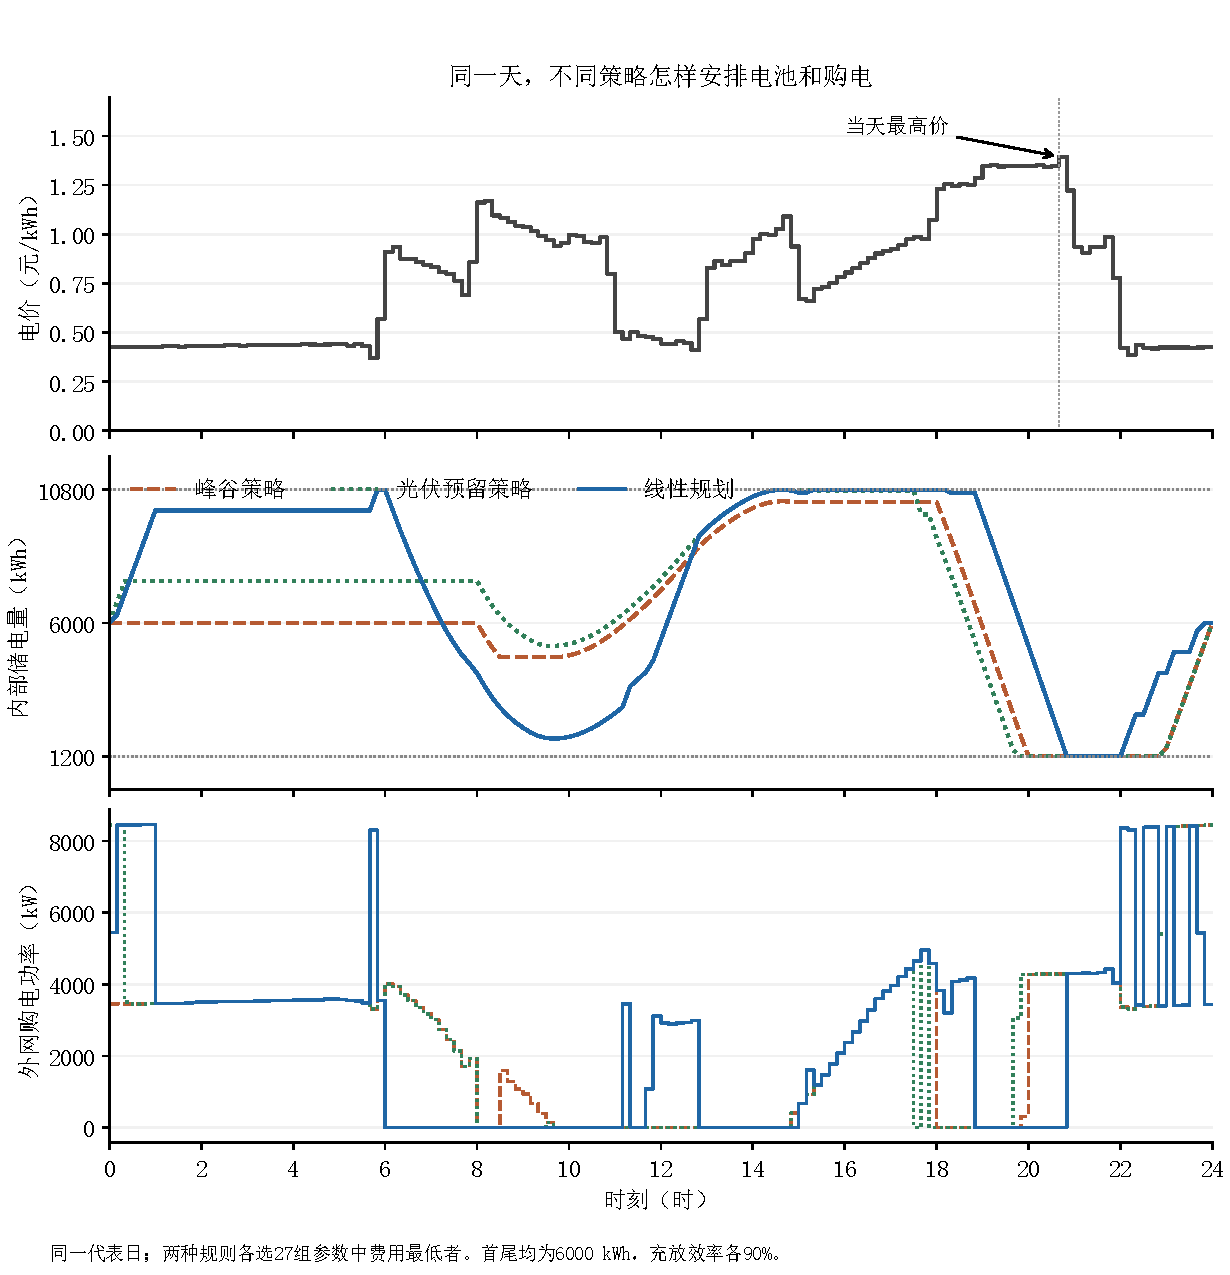
\includegraphics[width=0.90\linewidth]{q1_daily_dispatch.pdf}
 \caption{三种策略在相同代表日下的购电与储能安排}
 \label{fig:dispatch}
\end{inlinefigure}

\subsubsection{模型检验与初始储电量敏感性分析}
首先按导出的10分钟结果独立复算供需平衡、储电递推、容量与功率上限及全天费用，并核对首尾电量。三个起点案例的最大储电递推残差约为$1.34\times10^{-12}$ kWh；由求解器对偶信息独立重算的费用下界与实际可行方案费用之差最大约为$1.22\times10^{-12}$元。可行费用与下界在数值精度内一致，支持所列线性规划的最优性判断。此外，通过同价充放无套利、低高价两段充放以及初始库存不能免费消耗的小例子核对损耗与边界表达，并将导出表按真实时间逐项对应，避免零点置末造成结果错位。

问题一要求首尾电量相同，但相同的起点数值仍可能影响当天安排。为考察这种影响，保持供需、电价、效率和设备条件不变，分别以1200、6000和10800 kWh开始，每种情况均重新优化，并在日末恢复到各自起点。所得费用分别为\LowInitialCost{}元、\MainCost{}元和\HighInitialCost{}元；相较6000 kWh主方案，两个边界起点分别增加\LowInitialDelta{}元和\HighInitialDelta{}元，增幅为\LowInitialPct{}\%和\HighInitialPct{}\%。

三个案例的全天购电、累计充放电和光伏利用量相同，20点也都保留约\EveningState{} kWh，并避开最高价区间购电。但费用接近不表示逐段安排不变：两个替代起点各有14段购电量改变，均将5333.33 kWh从一部分时段转移到另一部分时段。低起点少了4800 kWh内部库存，凌晨需要多买$4800/0.9=5333.33$ kWh补充，日末则相应少补；高起点虽能减少凌晨补电，却必须在日末恢复更多库存。受充电功率和剩余时间限制，高起点还需在21:50--22:00以0.7764元/kWh额外购买666.67 kWh，因而开始时电量更多并不保证全天费用更低。

这三个已检验起点下，重新安排后的费用差异均不到1\%，且为晚间高价时段留电的特征保持一致；初始电量主要改变凌晨与日末的补电分配。检验只覆盖这三个取值，不能据此认定6000 kWh是整个允许区间内的最佳起点，也不能将重新优化后的结果解释为固定计划能够抵抗供需预测误差。问题一给出的是已知代表日下的调度依据；实际供需偏差出现后，计划与执行之间的差异还需在后续问题中处理。


\graphicspath{{q2_figures/}}
\section{问题二的模型建立与求解}
\subsection{未知供需下的日前购电安排}

问题一根据给定的一天供需曲线安排购电。问题二的困难在于，当天用多少电、光伏能发多少电，在零点都还没有发生，但普通购电量必须先确定。少买的部分可能要用五倍电价补购；多买的电若用不掉、也存不下，仍然需要付款。因此，本问要在提前多作准备的费用与临时补电的风险之间作出取舍。

为此，我们先把方案分成三层比较。第一层直接用历史同期数据预测，优点是规律清楚、首日以后即可滚动使用；第二层分别用岭回归和提升树预测负载与光伏，用来检验更复杂的拟合能否带来实际节费；第三层在历史预测上增加误差准备，专门防范少估缺口后产生的五倍紧急电费。问题二的核心损失并不对称：多订1 kWh通常只多付普通电费，少订1 kWh却可能支付五倍价格。因此，我们预先判断，单纯追求预测误差最小未必合适，能够根据近期误差主动留出准备量的方案更贴合题意。

最终建立的模型命名为：

\textbf{周期预测--近期加权准备--跨日线性规划模型。}

该模型先分别估计负载和光伏，再根据过去的预测偏差增加适量准备，最后安排外网购电和储能。白天普通订单保持不变，电池按实际供需补缺或充电，剩余缺口才由紧急购电补齐。这样既沿用问题一的电量平衡和设备限制，又能反映提前订电与实际用电之间的差别。

\subsection{负载与光伏的分别预测}

负载的星期规律较强，光伏则更受近期发电水平影响。若只预测二者的差值，容易把不同来源的变化混在一起。因此，分别用同星期历史估计负载，用近期历史估计光伏。以 $d$ 表示自然日，$k=1,\ldots,144$ 表示日内时段，每段长 $\Delta t=1/6$ 小时，第1段从0:00开始，第144段到24:00结束。$L_{d,k}$、$V_{d,k}$ 分别为负载和光伏功率，单位为 kW。历史充足时，预测为
\begin{equation}
\widehat L_{d,k}=\frac14\sum_{j=1}^{4}L_{d-7j,k},\qquad
\widehat V_{d,k}=\frac17\sum_{j=1}^{7}V_{d-j,k}.
\label{eq:q2-forecast}
\end{equation}
也就是说，负载参考过去四个相同星期的同一时刻，光伏参考最近七天的同一时刻。选中的负载历史各占四分之一，光伏历史各占七分之一。历史不足时按已有记录取平均；尚无可用记录的启动处理见第5节。

式\eqref{eq:q2-forecast}只使用当天零点以前的数据。附件2虽然保存了全年实际值，但当天及其后的真实值不参与当天预测。本问也不使用附件3的光伏预报。后面规划中涉及次日时，负载改为匹配次日的星期，光伏仍参考当前零点之前的七天，不能提前读入当天实际发电。

\subsection{根据近期误差确定准备量}

平均预测给出了通常的供需水平，却未必能应对连续几段的低估。电池能够补一段缺口，连续补电后仍可能达到储电下限。为减少这种情况，考察过去究竟把缺口看小了多少，并将其作为订电的准备依据。

对过去日期 $i$，按该日零点可获得的信息重建预测，定义净供需误差
\begin{equation}
\epsilon_{i,k}=\big[(L_{i,k}-V_{i,k})-(\widehat L_{i,k}-\widehat V_{i,k})\big]\Delta t.
\label{eq:q2-error}
\end{equation}
正值表示实际比预计更缺电，负值表示预计偏保守，单位均为 kWh。负载和光伏在预测时分开，在这里合并误差，是为了保留二者可能相互抵消、也可能共同扩大缺口的关系。

将一天分为六个4小时组，在最近28天中收集同组误差。较早的误差仍有参考价值，但近期供需已经改变时，不宜让旧记录占据同样分量。因此，对组内日期 $i$ 的每个时段赋予权重
\begin{equation}
\omega_{d,i,k}=\frac{\beta^{d-1-i}}
{\displaystyle\sum_{(j,u)\in\mathcal E_{d,g}}\beta^{d-1-j}},\qquad (i,k)\in\mathcal E_{d,g},
\label{eq:q2-weight}
\end{equation}
其中，$\mathcal E_{d,g}$ 是当天零点以前、最近28天第 $g$ 组的误差集合。$\beta$ 控制旧记录的权重下降速度。取 $\beta=0.7$ 时，最近一天、前一天和再前一天的相对权重依次为1、0.7和0.49，权重约每1.94天减半；按权重集中程度折算，所利用的信息量约相当于5.67个等权日期。也就是说，28天窗口仍覆盖四个星期，但真正主导准备量的是近期约一周的误差。同一天同组内各时段等分该日权重。

再将误差从小到大排列，取加权累计比例达到 $\alpha$ 的位置，并将负值截为零。写成
\begin{align}
F_{d,g}(u)&=\sum_{(i,k)\in\mathcal E_{d,g}}\omega_{d,i,k}\,\mathbf{1}\{\epsilon_{i,k}\le u\},\\
b_{d,k}&=\max\left\{0,\inf\{u:F_{d,g(k)}(u)\ge\alpha\}\right\}.
\label{eq:q2-margin}
\end{align}
$\mathbf1$ 在条件成立时取1，否则取0；$g(k)$ 表示时段 $k$ 所属的4小时组。采用 $\alpha=0.7$。它是误差排序的位置，与 $\beta$ 的时间权重含义不同，也不表示多买70\%的电或供电可靠率达到70\%。

准备量 $b_{d,k}$ 加在预测净需求上，由后续调度统一安排。它可能增加普通购电，也可能减少预计用于充电的光伏富余，或者改变电池放电时机，因而不是每段直接追加同样数量的订单。负误差也参与排序，避免只保留缺电记录而把准备量系统性抬高。

\subsection{购电与储能调度模型}

\textbf{决策变量。} 为兼顾午夜之后的用电，每天零点向前规划48小时，共288段，仅固定当天前144段的普通订单。以下以 $t$ 表示这两天中连续排列的时段。先由预测和准备量算出
\begin{equation}
r_t=(\widehat L_t-\widehat V_t)\Delta t+b_t,\qquad
n_t=\max(r_t,0),\quad a_t=\max(-r_t,0).
\end{equation}
$n_t$ 是需要外网或电池补充的电量，$a_t$ 是考虑准备量后预计可用于储存的富余。二者都是给定量。令 $x_t$ 为外网用于充电的电量，$y_t$ 为光伏用于充电的电量，$z_t$ 为电池送给负载的电量，$S_t$ 为段末内部储电量。前三者按设备外侧计量，$S_t$ 按内部计量，单位均为 kWh。普通订单为
\begin{equation}
q_t=n_t-z_t+x_t.
\label{eq:q2-order}
\end{equation}
式\eqref{eq:q2-order}表示：剩余负载先扣除电池能提供的部分，再加上主动购买的充电电量。外网可以直接供负载，也可以在低价时为电池充电。

\textbf{目标函数。} 计划费用按固定日内电价 $p_t$ 计算，两个规划日重复使用同一电价曲线。为给规划期末的余电保留一个未来使用的参考价值，目标取为
\begin{equation}
\min\ J=\sum_{t=1}^{288}p_tq_t-\nu S_{288},\qquad
\nu=0.9p_{00:00}=0.38484.
\label{eq:q2-objective}
\end{equation}
内部1 kWh电量最多向负载输出0.9 kWh，因此用0.9倍参考电价估计其价值。该项只帮助比较计划，不是售电收入，最终费用中不扣除它。真实的紧急购电尚不可知，这里以误差准备量应对其风险；方案好坏仍按实际发生的普通与紧急电费评价。

\textbf{约束条件。} 充电和放电效率各为90\%，储电量按
\begin{equation}
S_t=S_{t-1}+0.9(x_t+y_t)-\frac{z_t}{0.9},\qquad
1200\le S_t\le10800
\label{eq:q2-storage}
\end{equation}
逐段衔接。充入100 kWh，内部增加90 kWh；若向负载送出90 kWh，内部需减少100 kWh。充放电量还须满足
\begin{equation}
\begin{aligned}
&x_t\ge0,\qquad 0\le y_t\le a_t,\qquad q_t\ge0,\\
&x_t+y_t\le5000\Delta t,\qquad
0\le z_t\le\min\{n_t,5000\Delta t\},\quad t=1,\ldots,288.
\end{aligned}
\label{eq:q2-bounds}
\end{equation}
这里的5000 kW是电池的充、放电功率限制，换成10分钟电量后，每段外侧充电或放电最多833.33 kWh。$y_t\le a_t$ 防止储存不存在的光伏富余，$z_t\le n_t$ 防止向负载送出超过其需求的电。

$S_0$ 取当天实际剩余电量，不再要求每天首尾相等。给定预测与准备量后，式\eqref{eq:q2-order}--\eqref{eq:q2-bounds}构成连续线性规划，使用 HiGHS 求解。正电价下，同时用外网充电又向负载放电只会多付转换损耗，最优计划可避免这种动作；保存的求解结果也未出现同段同时充放。线性规划的最优性针对给定预测下的计划，并不等于已知未来真实供需时的最低全年电费。

\subsection{每日求解、实际供电与跨日运行}

每天零点先更新历史数据和电池库存，依次求出预测、准备量及普通订单。白天按10分钟区间检查实际供需。设本段负载和光伏电量为 $l$、$v$，按光伏优先直供的运行假设，直供量为 $m=\min(l,v)$，剩余负载为 $h=l-m$，光伏富余为 $a=v-m$。这里的优先顺序是采用的运行方式。

若 $h>q$，先用电池补充，在库存和放电功率允许范围内尽量满足当前缺口：
\begin{equation}
z=\min\{h-q,5000\Delta t,0.9(S-1200)\},\qquad e=h-q-z.
\label{eq:q2-emergency}
\end{equation}
$S$ 是本段开始的内部库存，$e$ 是紧急购电量，此段不充电，即 $x=y=0$。这说明即使电池里还有电，放电速度不够快也可能需要补购；达到1200 kWh下限时，则不能继续放电。

若 $h\le q$，将实际可利用的余电送入电池，总充电量为
\begin{equation}
c=\min\left\{a+q-h,5000\Delta t,\frac{10800-S}{0.9}\right\}.
\end{equation}
其中先使用光伏富余，即 $y=\min(a,c)$，其余 $x=c-y$ 由普通购电提供；本段不放电、不紧急购电。存不下的光伏不产生收入，未利用的普通订单仍照量付款。实际充放电再按式\eqref{eq:q2-storage}更新库存。这里用当前区间的实际功率代表区间内供需，作10分钟尺度的反馈近似，而非提前将全天实际值告知零点计划。

一天结束后，费用和次日初值分别为
\begin{equation}
C_d=\sum_{k=1}^{144}\left(p_kq_{d,k}+5p_ke_{d,k}\right),\qquad
S_{d+1,0}=S_{d,144}.
\label{eq:q2-bill}
\end{equation}
五倍电价仅作用于真正不足的紧急补购。当天普通订单不重新优化，实际充放电可以随当前供需变化；第二天零点再利用新积累的历史制定下一份订单。

全年从1月1日零点的6000 kWh连续运行。首日没有更早历史，普通订单采用问题一保留的购电安排。原实际序列缺少1月1日首个10分钟区间，仅该区间借用附件1的午夜参考值，并排除出预测训练记录。1月2日起采用固定的同星期负载、近三天光伏参考启动，历史不足时依次回退到可用的同刻记录，完全没有记录时才用附件1参考。1月末完成参数比较，所选参数从2月起使用，不倒填回1月的实际决策。2月1日零点库存由此得到8592.69 kWh，各候选均从这一共同状态开始比较。计算按真实日期和区间起点排序，00:10对应00:10--00:20；次日零点保留在次日，避免将表格最后一行误当成当天第一段。

\subsection{参数依据与方案比较}

选方案时，首先比较实际电费。预测误差较小固然有利，但同样大小的误差若集中出现在高价时段，或者连续耗掉电池可用电量，就可能带来更高的紧急费用。因此，除历史分别预测外，还比较了负载和光伏分别使用岭回归、提升树的方案，以及在历史预测上增加误差准备的方案。岭回归用受约束的线性关系组合历史信息，提升树则通过逐步修正预测来表达非线性变化。各方案使用相同电价、设备、起始库存、规划长度和实际供电规则。

预测窗口先在1月份比较负载1周或4周、光伏3天或7天的四种组合，选取4周和7天。$\alpha=0.7$ 是1月三档正准备量设置中费用最低的一档，但当月不加准备量的费用更低，说明准备量是否值得付费仍取决于后续供需变化。在全年误差诊断中发现旧记录可能拖慢反应后，进一步引入近期权重。

$\beta$ 的选择既要让模型跟得上近期变化，又要避免只被某一两天的异常带着走。若取更大的0.8或0.9，旧误差衰减较慢，季节或天气已经变化后，早期记录仍会过多影响当天准备量；完整回算中，两者分别比0.7多花约6.12万元和20.49万元。若继续减小，例如取0.6，等效样本量会降到约4天，准备量更容易被最近一个异常日推动而上下跳动。由于本次没有实跑小于0.7的全年费用，本文不把这一判断写成数值最优性，而把0.7解释为“较快适应近期变化”和“仍保留足够历史信息”之间的折中。这里的权重只表示历史记录离现在有多远，不是用熵权法给负载、光伏分配重要性，也不是把预测值乘以0.7。

虽然上述题意分析使我们优先考虑“历史预测加近期准备”，仍不能只靠直觉确定模型。表\ref{tab:q2-compare}给出2月1日至12月31日334天的同条件实跑费用，用实际普通电费与紧急电费检验这一选择。
\begin{inlinetable}
\caption{不同方案的334天实际购电费用（万元）}\label{tab:q2-compare}
\begin{tabular}{lrrr}\toprule
方案 & 普通电费 & 紧急电费 & 总电费\\\midrule
\tableinput{q2_tables/comparison.tex}
\bottomrule\end{tabular}
\end{inlinetable}

加入误差准备后，普通购电支出增加，但临时高价补购减少得更多。进一步将等权改为近期加权后，普通电费增加约1.97万元，紧急电费减少约46.63万元，净节省44.66万元，降幅为3.18\%。与不加准备量的历史预测方案相比，节省234.90万元，降幅为14.74\%。为分清改进来源，还统一了两者取分位数的方法；在相同取法下，近期权重仍节省44.54万元，主要收益确实来自对近期误差的重视。

提升树虽然降低了负载平均预测误差，却没有取得最低电费。这说明本题更需要把预测偏差对实际供电的影响纳入安排，而非单独追求预测曲线更贴近真实值。岭回归结构稳定，但难以单独表达天气和用电变化造成的局部偏差；提升树可以学习非线性，却没有直接处理五倍补购带来的损失不对称。近期加权准备恰好针对这一风险，并且保留了历史周期预测容易说明、容易滚动更新的特点。因此，候选比较不仅验证了它的费用更低，也验证了最初依据题意作出的结构选择。

该比较针对表中的具体组合，并未把回归、树与各种准备量全部交叉试验；历史窗口也存在更便宜的短窗口对照。因此，这里的选择有实际费用依据，但不意味着其他预测方法或所有参数组合都已被排除。

\subsection{全年结果与指定日期分析}

题目要求的2--12月共334天，总费用为\textbf{13583810.84元}，其中普通电费12979560.57元，紧急电费604250.27元。若计入共同启动的1月份，连续365天费用为15709745.62元。以下比较均采用334天范围，完整逐段结果保存于 \texttt{result2.xlsx}。

为判断节费是否仅来自少数月份，图\ref{fig:q2-monthly}同时展示月度费用构成和相对等权准备方案的节省。
\begin{inlinefigure}
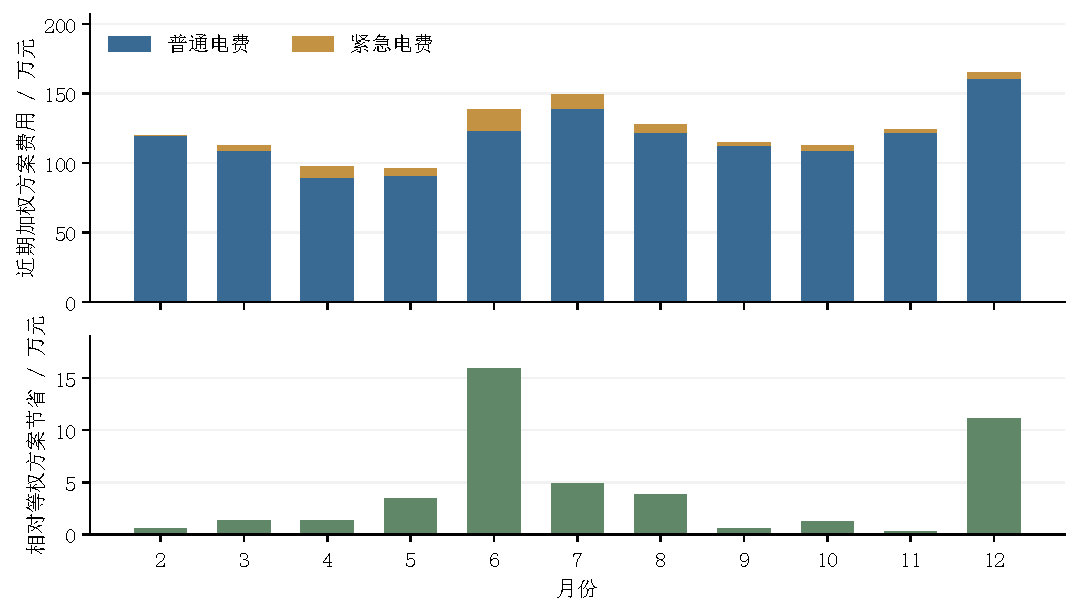
\includegraphics[width=.96\linewidth]{monthly_cost.pdf}
\caption{近期加权准备方案的月度费用及相对等权准备的节省}\label{fig:q2-monthly}
\end{inlinefigure}
11个月合计均有所节省，但收益并不均匀，6月和12月贡献较多。这说明近期误差对订电的参考价值随供需变化而变化。月度节省也不代表每天更便宜：逐日比较中195天节省、135天增加、4天相同。6月3日最多节省32898.37元，6月24日则多支出19484.15元，反映出近期权重在减少缺口的同时也可能跟随短暂波动而多订电。

按题目指定日期，表\ref{tab:q2-purchase}列出六个10分钟区间的计划购电量，以及全天购电和费用。各日总量取完整144段合计，不能由展示的六段相加代替。普通订单即使未实际利用也计入购电量和费用，紧急补购另列后汇总。
\begin{inlinetable}
\caption{指定日期的计划购电及全天费用（电量单位：kWh）}\label{tab:q2-purchase}
\begin{tabular}{lrrrr}\toprule
区间或项目 & 3月20日 & 6月21日 & 9月23日 & 12月21日\\\midrule
\tableinput{q2_tables/purchase.tex}
\bottomrule\end{tabular}
\end{inlinetable}

储能的实际运行见表\ref{tab:q2-storage}。充放电量按设备外侧计量，日首尾库存按设备内部计量，两者通过90\%的充、放效率衔接。一个4小时区间内既有充电又有放电，是因为不同10分钟段采取了不同动作，并不表示同段同时充放。
\begin{inlinetable}
\caption{指定日期的实际充放电量及日首尾储电量（kWh）}\label{tab:q2-storage}
\begin{tabular}{llrrrr}\toprule
区间 & 项目 & 3月20日 & 6月21日 & 9月23日 & 12月21日\\\midrule
\tableinput{q2_tables/storage.tex}
\bottomrule\end{tabular}
\end{inlinetable}

四个指定日期中，两天发生紧急购电，时间、电量和费用见表\ref{tab:q2-emergency}。6月21日和12月21日无紧急补购，说明供需预测存在偏差时，也可能由普通电和电池共同消化。
\begin{inlinetable}
\caption{指定日期的紧急购电}\label{tab:q2-emergency}
\begin{tabular}{llrr}\toprule
日期 & 发生区间 & 电量 / kWh & 费用 / 元\\\midrule
\tableinput{q2_tables/emergency.tex}
\bottomrule\end{tabular}
\end{inlinetable}

为说明电池怎样缓冲偏差，从题目指定日期中选取有紧急补购的3月20日和无紧急补购的6月21日，见图\ref{fig:q2-days}。上图对照供需和订单，中图追踪实际库存，下图显示普通电之后的缺口由谁补齐。
\begin{inlinefigure}
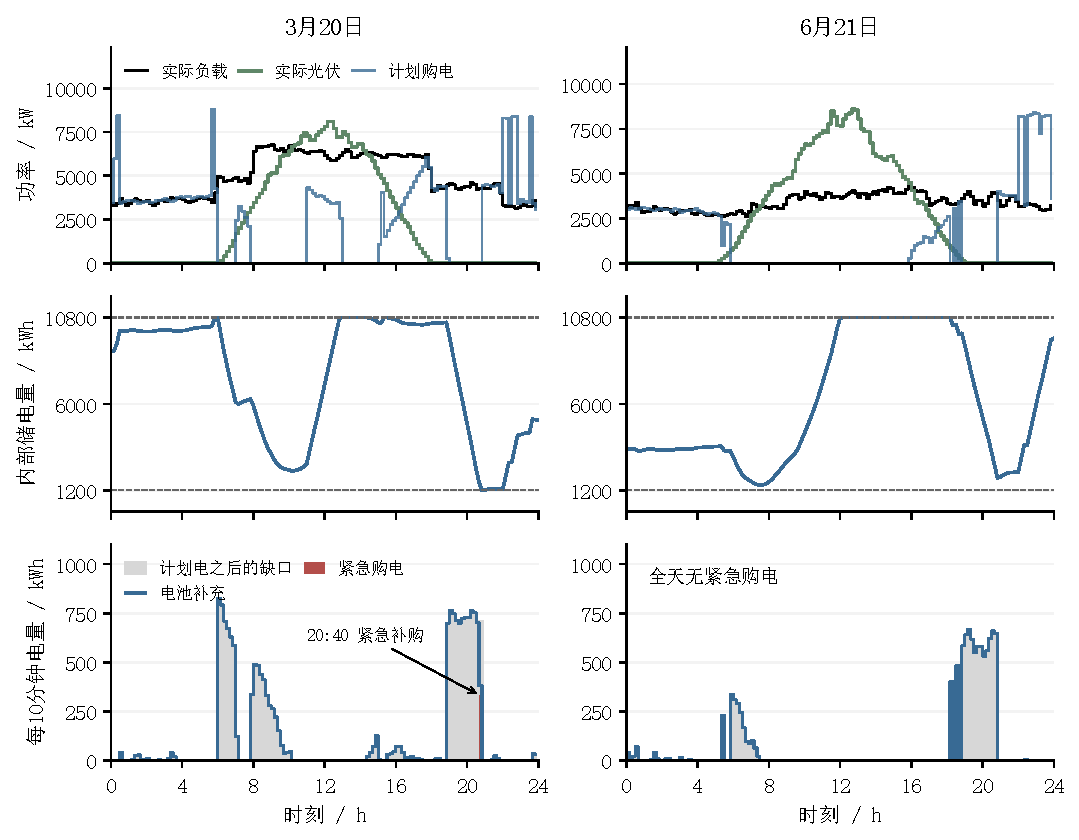
\includegraphics[width=.98\linewidth]{specified_days.pdf}
\caption{两个指定日期的供需、库存与缺口补充；虚线为储电上下限}\label{fig:q2-days}
\end{inlinefigure}
3月20日的大部分缺口由电池补充，但20:40开始时内部库存仅1622.06 kWh，补电后达到1200 kWh下限，剩余329.52 kWh只能紧急购入。6月21日则通过白天吸收光伏和跨时段放电，全天未发生紧急补购。两天的差别说明，判断能否按时供电，需要同时看每段缺口、电池剩余电量和放电能力；全天总电量够用并不足以作出判断。这两个日期用于解释运行过程，全年优劣仍由完整334天比较确定。

\subsection{灵敏度检验与风险分析}

准备量是否越大越好，需要看多付的普通电费能否换来更多的紧急费下降。图\ref{fig:q2-sensitivity}分别改变分位位置 $\alpha$ 和衰减参数 $\beta$，其余设置保持不变，费用变化均以 $\alpha=\beta=0.7$ 为参照。
\begin{inlinefigure}
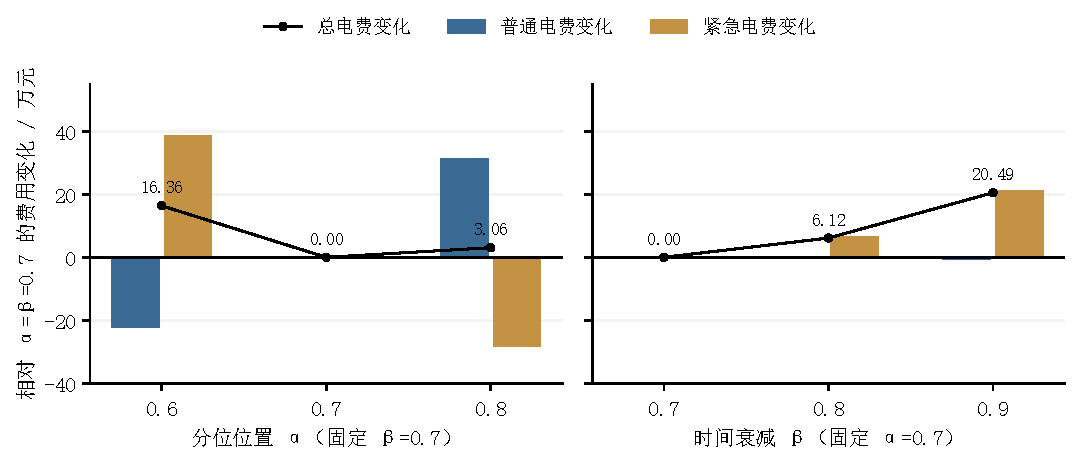
\includegraphics[width=.97\linewidth]{sensitivity.pdf}
\caption{准备程度与近期权重的费用影响（2025年2--12月）}\label{fig:q2-sensitivity}
\end{inlinefigure}
将 $\alpha$ 从0.7提高到0.8后，紧急购电天数由156天降至102天，但普通电费的增加超过紧急电费的减少，总费用反而增加约3.06万元；降到0.6时，准备不足使总费增加约16.36万元。$\beta$ 从0.7提高到0.8或0.9后，旧误差保留更久，本次费用分别增加约6.12万元和20.49万元。因此，所试设置支持保留0.7附近的准备程度和较快的近期反应，并不证明连续参数范围内存在唯一最优点。

规划长度也有取舍。改为只看24小时后，总费用低3215.61元，差异约0.024\%，但紧急购电天数增加，最长连续紧急补购由200分钟延长至340分钟，年末库存也明显减少。故保留48小时是费用相近时对跨日库存和紧急风险的权衡。去掉式\eqref{eq:q2-objective}的期末参考价值后，本次实际总费用未变，不能将它单独视作已证实的节费来源。

逐段复核了预测可用信息、电量平衡、设备限制、跨日库存和费用，结果相互一致。方案仍有156天需要紧急购电。其中，有的时段已达到最低库存，有的则受到放电功率限制，说明储能能够缓冲偏差，却无法消除全部预测风险。

为考察连续偏差是否会改变选择，再用过去已有的三天误差片段，分别构造持续低估负载、高估光伏及二者同时发生的情景。\footnote{每14天安排一次三天情景，从此前28天合格片段中按不利误差的90\%最近秩选取；该日程和排序位置均不表示真实发生概率。负载及联合情景实际扰动各45天，光伏72天；部分月份缺少合格片段，未额外补造扰动。}三类所测情景下，总费用仍比等权方案低3.09\%--3.52\%，说明近期准备的总体节费作用在这些偏差下得以保留。但短时波动也可能使其多订电，单日仍会失利。以上结论来自一个年份，方法选择也参考过全年诊断，因此支持本题数据下的应用，尚不足以保证在新年份或其他小区同样有效。


\graphicspath{{q3_figures/}}
\section{问题三的模型建立与求解}
\subsection{日内新信息怎样改变购电决策}

问题二只能在每天零点制定一次购电计划，白天即使发现光伏偏离预期，也不能修改普通订单。问题三允许在6:00、12:00和18:00收到新光伏预报后，重新安排尚未执行的部分。因此，本问的关键不只是把预报做得更准，还要判断修改订单能否抵消调整费，并让电池在新旧计划之间平稳衔接。

我们把一天划分为144个10分钟区间，记日期为 $d$，日内区间为 $k=1,\ldots,144$，每段长度为 $\Delta t=1/6$ 小时。第1段对应0:00--0:10，第144段对应23:50--24:00。零点形成当天原计划，6:00、12:00和18:00分别在第37、73和109段开始前更新；已经过去的区间保持不变，只调整未来订单。附件2中的实际负载和实际光伏只在相应时段结束后成为历史信息，附件3才是各发布时间能够看到的未来光伏预报。

新预报并不意味着每次改单都划算。如果预报只发生小幅变化，节省的购电量可能还不够支付调整费；如果电池已经存有足够电量，也可能无需改约。为选出与这种信息结构相符的方案，我们设置四个候选：直接使用官方预报；用历史误差融合官方预报；用提升树修正官方预报；在融合预报上再加入近期误差准备。四个候选都接入相同的日内滚动调度，因而能够把预报方法的差别落实到最终电费上。

官方预报给出了当天最直接的信息，但它按小时发布且仍有误差；近期同刻历史能补充稳定规律，却不能替代当天预报；提升树可以表达非线性，但较难直接说明每次修正来自哪里。另一方面，少估缺口会触发五倍紧急电费，所以模型还必须专门处理低估风险。基于这些特点，我们预先选择“历史融合＋动态准备＋滚动规划”作为主方案，再用全年费用检验这一判断。最终模型命名为：

\textbf{历史融合预报--动态安全准备--日内滚动规划模型。}

\subsection{用历史记录修正光伏预报}

负载和光伏的形成规律不同，因此仍然分开估计。负载沿用问题二的同星期历史参考：以过去四个相同星期的同一时刻均值作为基础预测。光伏则先读取附件3在当前时点发布的预报，再用此前已经兑现的实际光伏判断这份预报应当相信多少。

附件3按整点给出预测，而购电计划按10分钟填写。对同一发布时间的相邻两个整点预测采用线性插值，将其转换为10分钟功率。该处理保留了整点值和相邻时刻的变化方向，只是把小时信息平滑分配到10分钟尺度，并不把插值结果当作新获得的真实观测。

记当前发布时间为 $r$，附件3给出的光伏预测为 $F_{r,t}$，最近七个可用同刻实际值形成的历史参考为 $H_{r,t}$。将未来24小时按提前1--6、7--12、13--18和19--24小时分组，在每一组中用过去28天、且在发布时间 $r$ 前已经能够核验的样本确定融合权重：
\begin{equation}
\widehat V_{r,t}=w_{r,g}F_{r,t}+(1-w_{r,g})H_{r,t},
\qquad 0\le w_{r,g}\le1,
\label{eq:q3-fusion}
\end{equation}
\begin{equation}
w_{r,g}=\operatorname{clip}_{[0,1]}
\frac{\sum_{j\in\mathcal H_{r,g}}(F_j-H_j)(V_j-H_j)}
{\sum_{j\in\mathcal H_{r,g}}(F_j-H_j)^2}.
\label{eq:q3-weight}
\end{equation}
其中，$\mathcal H_{r,g}$ 只包含当时已经发生的历史记录。式\eqref{eq:q3-weight}选择使历史平方误差最小的权重：官方预报过去更可靠时，$w$ 自动增大；历史同刻曲线更可靠时，$w$ 自动减小。它会随发布时间和提前时长变化，并不是人为指定一个固定比例，也不是用熵权法分配权重。

\subsection{根据近期净需求误差留出准备量}

只提高光伏预测精度仍不能解决风险不对称的问题。少估1 kWh缺口，运行时可能要按五倍电价紧急补购；多准备1 kWh普通电，也可能因为负载较低或电池已满而无法利用。因此，我们不直接把订单整体放大，而是从近期净需求误差中估计每个时段应保留多少安全余量。

对过去已经兑现的记录，定义10分钟净需求误差为
\begin{equation}
\varepsilon_{i,k}=
\big[(L_{i,k}-V_{i,k})-(\widehat L_{i,k}-\widehat V_{i,k})\big]\Delta t.
\label{eq:q3-error}
\end{equation}
正值表示当时把缺电量看小了，负值表示计划偏保守。每次更新时，只使用此前28天的误差，并把一天分为8个3小时组。同组时段面对相近的光照和用电阶段，样本数量又足以支撑分位估计。

近期误差比很久以前的误差更能反映当前天气和用电水平。若样本 $j$ 距当前完整相隔 $a_j$ 天，赋予权重
\begin{equation}
\omega_j=\frac{\beta^{a_j}}{\sum_l\beta^{a_l}},\qquad \beta=0.7.
\label{eq:q3-decay}
\end{equation}
这表示最近一天的相对权重为1，再早一天为0.7，再早两天为0.49。其半衰期约为1.94天，既保留数周的可用记录，又让近期变化起主要作用。最后取同组误差的加权0.60分位，并把负值截为0：
\begin{equation}
m_{r,k}=\max\left\{0,Q_{0.60}^{(\omega)}(\varepsilon_{i,k})\right\}.
\label{eq:q3-margin}
\end{equation}
0.60高于中位数，是因为低估缺口的代价更高；它又没有取到过高位置，以免普通电准备过多。每次收到新预报后都重新计算并完整保留该准备量，而不是随着日内更新逐次撤掉。

\subsection{滚动购电与储能调度模型}

\textbf{预计供需。} 由负载预测 $\widehat L_t$、融合光伏预测 $\widehat V_t$ 和准备量 $m_t$ 得到
\begin{equation}
r_t=(\widehat L_t-\widehat V_t)\Delta t+m_t,\qquad
n_t=\max(r_t,0),\quad a_t=\max(-r_t,0).
\label{eq:q3-net}
\end{equation}
$n_t$ 表示预计仍需外网或电池补充的电量，$a_t$ 表示考虑准备量后预计能够储存的光伏富余。

\textbf{决策变量。} 令 $q_t$ 为普通购电订单，$x_t$ 和 $y_t$ 分别为外网充电量和光伏充电量，$z_t$ 为电池向负载送出的电量，$e_t$ 为规划中预留的紧急购电量，$u_t$ 为已经下单但预计无法接收的普通电量，$S_t$ 为区间结束时的内部储电量。除 $S_t$ 外，各变量均按设备外侧、每10分钟的 kWh 计量。

\textbf{供需与储能约束。} 光伏先直接满足负载，式\eqref{eq:q3-net}已经扣除了这部分直供量。其余电量满足
\begin{equation}
q_t-x_t+z_t+e_t-u_t=n_t.
\label{eq:q3-balance}
\end{equation}
普通电可以直接供负载，也可以通过 $x_t$ 给电池充电；若订单过多且电池存不下，则由 $u_t$ 记录未接收但仍需结算的部分。充、放电效率均为90\%，所以
\begin{equation}
S_t=S_{t-1}+0.9(x_t+y_t)-\frac{z_t}{0.9},qquad
1200\le S_t\le10800.
\label{eq:q3-storage}
\end{equation}
设备功率上限为5000 kW，换算到10分钟后，每段最多充入或放出 $5000\Delta t=833.33$ kWh：
\begin{equation}
\begin{aligned}
&x_t,y_t,z_t,e_t,u_t,q_t\ge0,\qquad y_t\le a_t,\\
&x_t+y_t\le5000\Delta t,\qquad z_t+e_t\le n_t.
\end{aligned}
\label{eq:q3-bounds}
\end{equation}
每天的初始库存取上一天24:00的实际剩余电量，不额外要求日首和日末相等。

\textbf{购电与调整费用。} 记零点确定的原订单为 $q_t^0$，执行前最后一次调整后的订单为 $q_t^F$。按照采用的结算口径，多个时点对同一时段的修改只看最终订单相对零点订单的净变化，不重复累计中间改单。普通结算与实际总费用分别为
\begin{equation}
C^{\rm ord}=\sum_t\left[p_tq_t^F+\frac12p_t|q_t^F-q_t^0|\right],
\label{eq:q3-ordinary}
\end{equation}
\begin{equation}
C=\sum_{d,k}\left[p_kq_{d,k}^F+\frac12p_k|q_{d,k}^F-q_{d,k}^0|
+5p_ke^{\rm actual}_{d,k}\right].
\label{eq:q3-bill}
\end{equation}
例如，原计划100 kWh、单价1元，后来减至80 kWh，则普通订单费为80元，调整费为10元，相关费用共90元；原计划的100元不再重复相加。

\textbf{目标函数。} 在每次决策时，对当前时刻至次日24:00进行规划，最小化预计普通购电、调整和紧急购电费用：
\begin{equation}
\min J=\sum_{t\in\mathcal T_r}
\left[p_tq_t+\frac12p_t\delta_t+5p_te_t\right]-\nu S_T,
\label{eq:q3-objective}
\end{equation}
\begin{equation}
\delta_t\ge q_t-q_t^0,qquad \delta_t\ge q_t^0-q_t,qquad
\nu=0.9p_{00:00}.
\label{eq:q3-absolute}
\end{equation}
$\delta_t$ 将绝对值调整费写成线性约束。末端库存项用于避免规划在边界前无节制地放空电池，$\nu$ 只代表余电未来可用价值，不作为售电收入计入式\eqref{eq:q3-bill}。

\subsection{模型求解}

给定某次发布时间能够获得的信息后，式\eqref{eq:q3-net}--\eqref{eq:q3-absolute}中的目标和约束都是线性的，因此采用线性规划求解。每个比赛日按以下顺序运行：
\begin{enumerate}
\item 零点读取当时已有历史、当前真实库存和当天光伏预报，将整点预报插值到10分钟，计算负载预测、融合光伏预测及误差准备量；
\item 从零点规划到次日24:00，保存当天前144段普通订单作为 $q^0$，次日部分只帮助安排跨日库存；
\item 6:00、12:00和18:00收到新预报后，以该时刻真实库存为新初值，重新计算未来预测和准备量；已经执行的订单锁定，只求解当天尚未执行的部分；
\item 执行接下来的6小时。实际光伏先供负载，剩余普通订单和光伏在功率、容量允许时充电；普通订单不足时先由电池补缺，仍不足的部分才紧急购买；
\item 24:00按最终订单相对零点订单的净变化结算，日末真实库存传给下一天。
\end{enumerate}

2月1日零点库存取1月连续运行得到的8592.69 kWh。2月1日至12月31日共334天，每天求解4次，合计1336次线性规划均得到可行最优解。最大约束残差为 $1.82\times10^{-12}$，最大对偶差为 $1.31\times10^{-10}$，说明保存的方案满足供需、库存和功率限制。

\subsection{从候选比较到最终策略}

前面的题意分析使我们优先选择历史融合、误差准备与滚动规划的组合，但这一预选仍需接受同条件检验。为避免只凭预测误差选模型，我们让各候选使用相同负载预测、设备参数、初始库存、实际供电规则和结算方法，只改变光伏处理和风险准备。表\ref{tab:q3-candidates}给出完整334天的实际费用。
\begin{inlinetable}
\caption{问题三候选方案的334天费用比较}\label{tab:q3-candidates}
\resizebox{\linewidth}{!}{\begin{tabular}{lrrrr}\toprule
方案 & 普通结算/万元 & 紧急购电/万元 & 总费用/万元 & 紧急购电天数\\\midrule
\tableinput{q3_tables/candidates.tex}
\bottomrule\end{tabular}}
\end{inlinetable}

直接采用官方预报的总费用为1417.51万元。利用历史误差融合后降至1408.87万元，说明官方预报和近期同刻记录确实能够互相补充。提升树虽然可以表达更复杂的非线性关系，但用于下一阶段决策的短期误差和最终费用都没有占优。更值得注意的是，初始融合方案的普通费用较低，紧急费用却达到132.51万元，说明“平均上更准”仍可能在少数关键时段低估缺口。

在融合方案上加入近期净需求误差准备后，总费用降为1314.65万元，比初始融合方案节省94.22万元。普通结算增加17.98万元，但紧急费用减少112.20万元，减少的高价补购远大于增加的普通准备。提升树能够表达复杂关系，但本题的官方预报已经提供了较强先验，树模型的短期修正没有换来更低费用；历史融合可以清楚说明官方预报与近期记录各起什么作用，再配合准备量处理高价缺口，结构上更符合题意。由此，费用结果与建模前的判断一致，最终采用\textbf{历史融合预报--动态安全准备--日内滚动规划模型}。

\subsection{全年结果与指定日期分析}

最终方案在334天内的普通结算为\textbf{12943484.52元}，紧急购电费为\textbf{203050.97元}，总费用为\textbf{13146535.49元}；紧急购电量为35685.12 kWh，共有164天出现过至少一个紧急购电区间。年末内部库存为8514.41 kWh。图\ref{fig:q3-monthly}显示，11个月相对初始融合方案都实现节省，主要收益来自减少紧急购电。
\begin{inlinefigure}
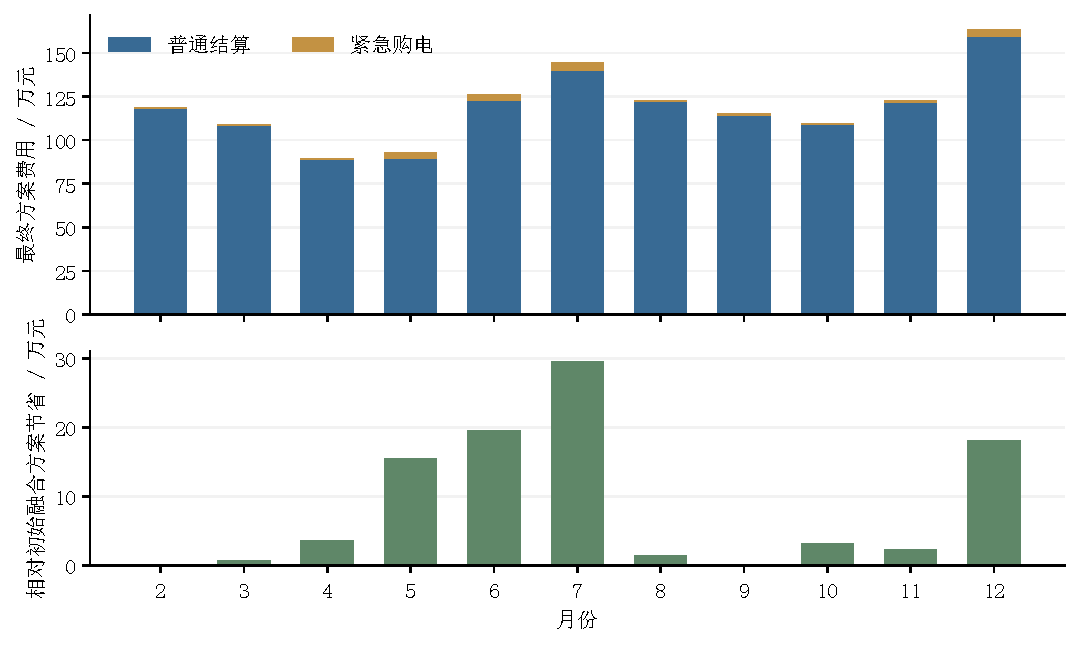
\includegraphics[width=.96\linewidth]{final_monthly.pdf}
\caption{最终方案的月度费用及相对初始融合方案的节省}\label{fig:q3-monthly}
\end{inlinefigure}

月度均有节省不代表每天都更便宜。逐日比较中，250天节省、59天增加、25天基本相同；7月7日最多节省23360.46元，6月29日则增加1041.73元。模型付出的代价还包括443358.10 kWh未接收普通订单，说明安全准备能够减少高价缺口，但不能被描述为没有代价的改进。

题目指定日期的零点原计划和调整后订单见表\ref{tab:q3-original}、表\ref{tab:q3-adjusted}。正文只列六个代表时段，全天总量按完整144段求和。
\begin{inlinetable}
\caption{指定日期零点原计划的部分时段购电量（kWh）}\label{tab:q3-original}
\resizebox{\linewidth}{!}{\begin{tabular}{lrrrr}\toprule
区间 & 3月20日 & 6月21日 & 9月23日 & 12月21日\\\midrule
\tableinput{q3_tables/original_orders.tex}
\bottomrule\end{tabular}}
\end{inlinetable}

\begin{inlinetable}
\caption{指定日期调整后订单及全天费用（电量单位：kWh）}\label{tab:q3-adjusted}
\resizebox{\linewidth}{!}{\begin{tabular}{lrrrr}\toprule
区间或项目 & 3月20日 & 6月21日 & 9月23日 & 12月21日\\\midrule
\tableinput{q3_tables/adjusted_orders.tex}
\bottomrule\end{tabular}}
\end{inlinetable}

表\ref{tab:q3-storage}汇总各4小时内的实际充放电量。一个4小时段内同时出现充、放电，表示其中不同10分钟区间采取了不同动作，并非同一时段同时充放。四天日末库存都直接传给次日，没有人为恢复到日初水平。
\begin{inlinetable}
\caption{指定日期的实际充放电及日首尾库存（kWh）}\label{tab:q3-storage}
\resizebox{\linewidth}{!}{\begin{tabular}{llrrrr}\toprule
区间 & 项目 & 3月20日 & 6月21日 & 9月23日 & 12月21日\\\midrule
\tableinput{q3_tables/storage.tex}
\bottomrule\end{tabular}}
\end{inlinetable}

四个指定日期都只出现少量紧急购电，具体时段见表\ref{tab:q3-emergency}。图\ref{fig:q3-days}进一步展示其中紧急量最大和最小的3月20日、9月23日。大部分普通订单后的缺口都由电池补上；3月20日20:40附近库存接近下限，仍有95.59 kWh无法由电池提供，只能紧急购入。9月23日仅在20:30出现6.38 kWh补购。可见是否需要紧急购电取决于缺口发生的具体时刻、当时库存和放电速度，不能只比较全天电量总和。
\begin{inlinetable}
\caption{指定日期的紧急购电明细}\label{tab:q3-emergency}
\begin{tabular}{llrr}\toprule
日期 & 发生区间 & 电量/kWh & 费用/元\\\midrule
\tableinput{q3_tables/emergency.tex}
\bottomrule\end{tabular}
\end{inlinetable}

\begin{inlinefigure}
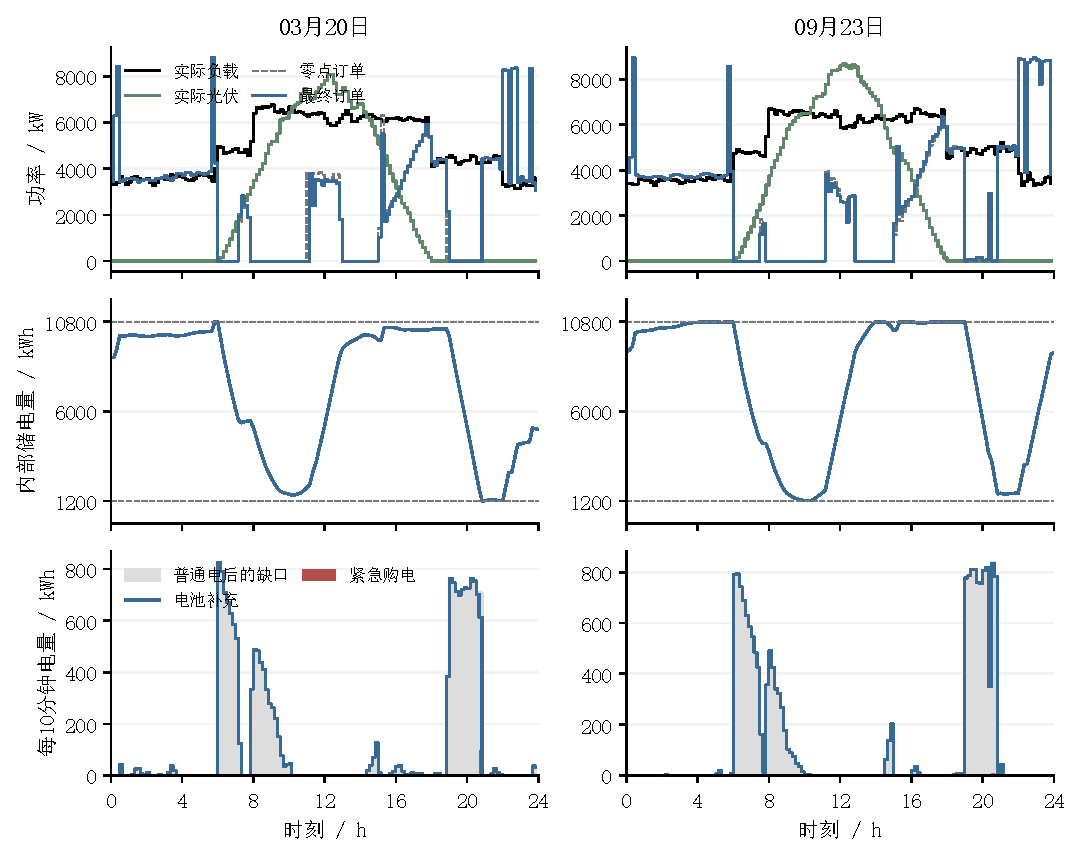
\includegraphics[width=.98\linewidth]{specified_days.pdf}
\caption{两个指定日期的供需、库存和缺口补充过程}\label{fig:q3-days}
\end{inlinefigure}

\subsection{日内预报带来的实际费用价值}

问题三要求评价日内预报的价值。若只把“零点全天不改订单”和“使用日内新预报”直接相减，会把实时看到实际供需、重新掌握电池库存以及允许改约的作用一并算进去。为分开这些影响，在直接采用官方预报的同一策略下设置三个逐步增加信息的对照：零点订电后全天不改；允许日内反馈和改约，但不读取后发官方预报；在此基础上再使用6:00、12:00、18:00的新预报。

如图\ref{fig:q3-value}所示，三种设置总费用依次为1614.80、1439.29和1417.51万元。开放日内反馈与改约先节省175.51万元，在此基础上使用新官方预报再节省21.78万元。前者体现“根据实际运行修正未来安排”的价值，后者才是新增官方预报在该对照顺序下带来的增量价值。两者合计197.28万元，不能全部归因于新预报。
\begin{inlinefigure}
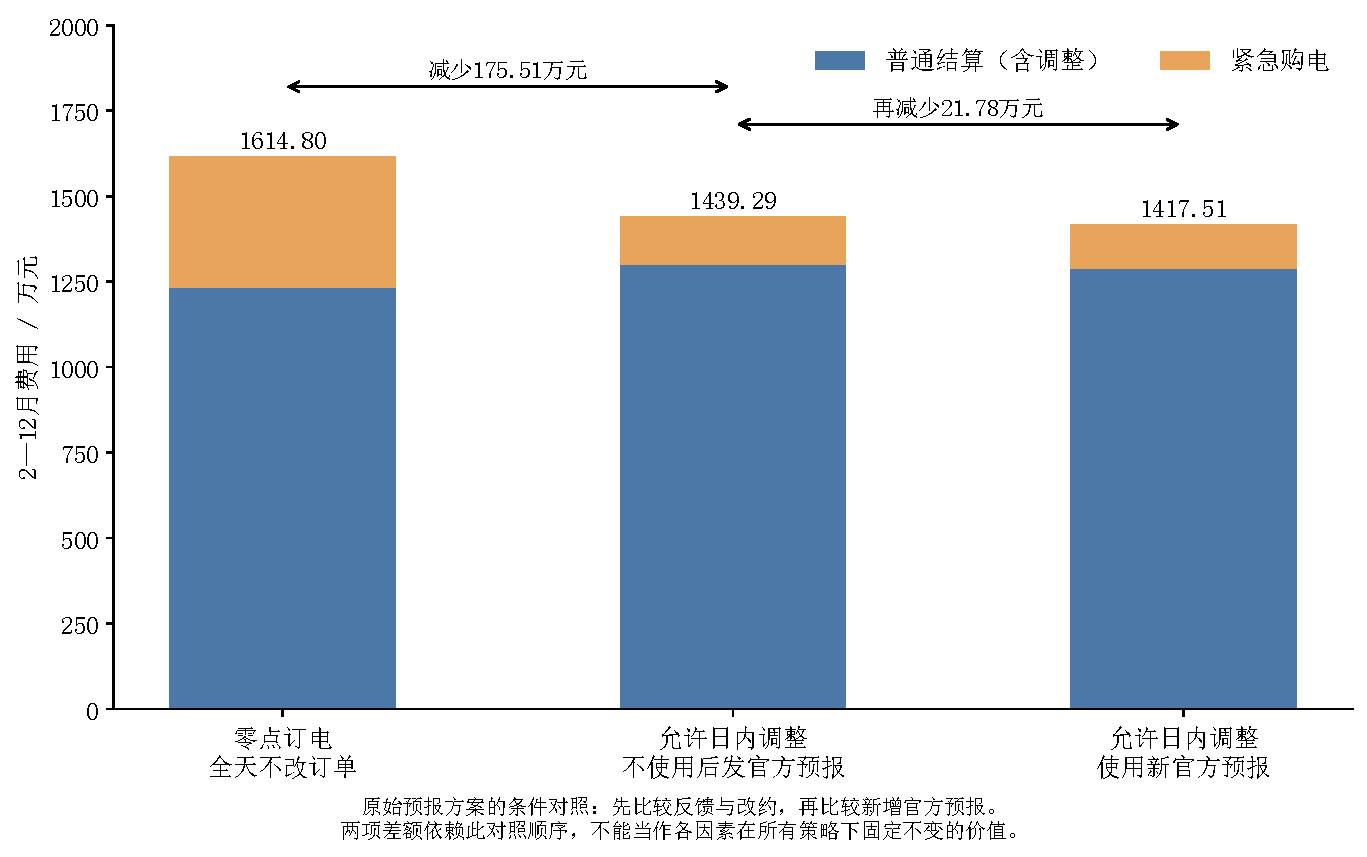
\includegraphics[width=.96\linewidth]{information_value.pdf}
\caption{日内反馈、改约与新增官方预报的费用价值}\label{fig:q3-value}
\end{inlinefigure}

因此，对题目最后提出的“是否需要引入6:00、12:00和18:00预报”这一问题，本文的回答是：\textbf{需要引入}。在日内反馈和改单权限完全相同的条件下，使用后发预报把费用从1439.29万元降到1417.51万元，额外节省21.78万元，约为1.51\%。这说明新预报总体上有实际价值，但不表示三个发布时间同样重要，也不表示每次收到预报都必须改单；模型仍应结合调整费、实际库存和未来缺口决定是否修改订单。

\subsection{参数灵敏度与模型可信度}

准备量越大，紧急补购通常越少，但普通订单和未接收电量会增加，因此参数不能只按“越稳越好”来取。图\ref{fig:q3-parameter}在其余条件相同时比较了误差分位、日期衰减、分组长度和历史窗口。

在0.55--0.80的分位范围内，0.60的总费用最低；继续提高分位虽然压低了紧急费用，却使普通结算增加得更多。日期衰减取0.7时费用明显低于0.8和1.0，说明近期误差应当发挥更大作用。1、2、3、4和6小时分组中，3小时最低，且正好把每个6小时更新区间分为两段，在细节和稳定性之间取得平衡。历史窗口从14天改为28天或56天时，费用只相差十余元，因此选择能够覆盖四个星期的28天。

\begin{inlinefigure}
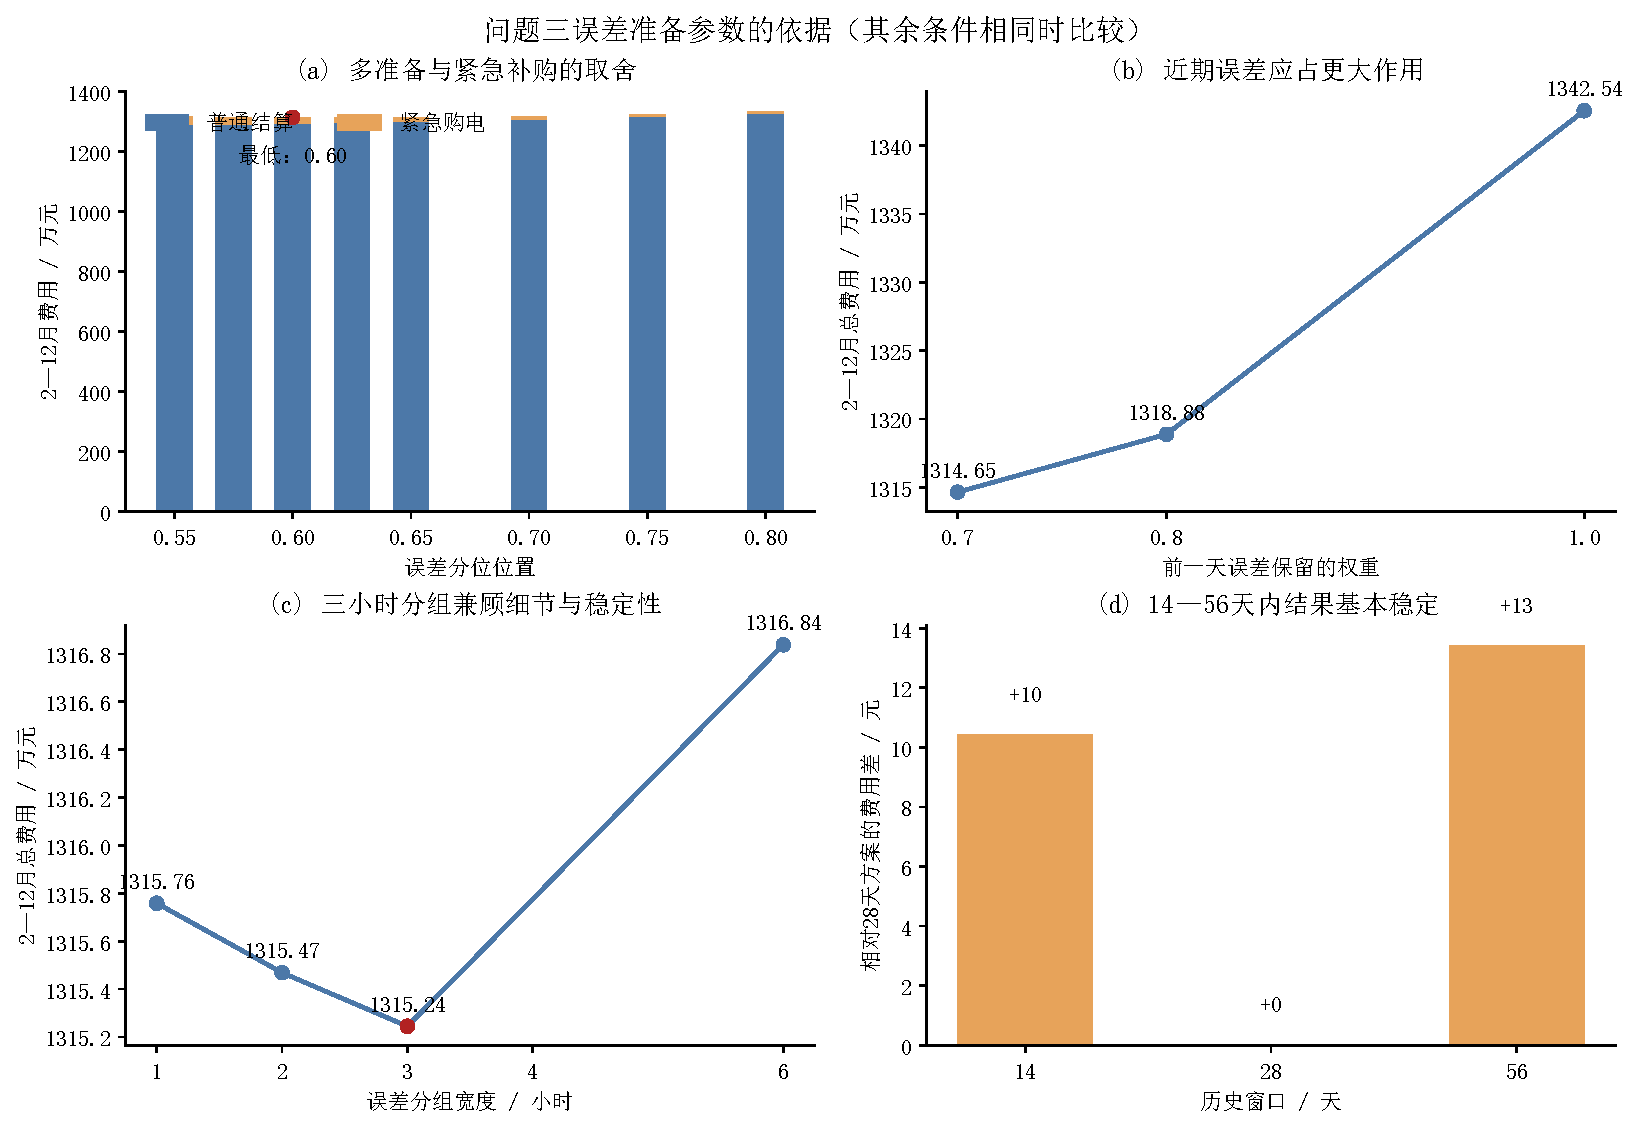
\includegraphics[width=.92\linewidth]{parameter_interpretability.pdf}
\caption{近期误差准备参数的费用依据}\label{fig:q3-parameter}
\end{inlinefigure}

此外，逐次撤去准备量、以及强制保留零点订单的25\%--100\%两类限制都会增加总费用，所以最终方案在四次决策中都保留完整准备量，也不给向下调整另设最低比例。这并不表示每次都必须改单，而是让式\eqref{eq:q3-objective}根据预报变化、调整费和真实库存自行判断。

为检查结果是否来自计算误差，对27条补充策略的1298592个实际10分钟区间和18980个准备量分组进行了独立回算。费用最大复算差约为 $1.9\times10^{-9}$ 元，库存、功率、订单锁定和逐段供需均满足约束。当前参数是在题目给出的2025年数据范围内比较得到，能够说明本年度的费用取舍和计算一致性；对于新的年份或不同小区，仍需用新数据重新校准，而不能直接认为同一组参数永远最优。


\graphicspath{{q4_figures/}}
\section{问题四的模型建立与求解}

\subsection{求解思路与模型选择}

问题四是在问题二、三的基础上进一步考虑外网电价的实时波动。前文已经解决了负载与光伏预测、误差准备、储能调度和订单调整问题，本问真正新增的困难是：制定订单时，未来各时段的实际电价也尚未发生。如果仍按固定电价安排储能，就可能在并不便宜的时段提前充电，或在后面更高的价格到来之前过早放空电池。因此，波动电价不仅改变最终账单，也会改变购电和充放电时点。

本问仍分为两种运行方式。对应问题二时，每天只能在0:00确定当天订单，之后即使电价判断发生偏差也不能改单；对应问题三时，6:00、12:00和18:00可以根据已经发生的价格、最新光伏预报和实际库存重新安排未执行订单。两种运行方式的信息条件不同，价格模型也不宜简单照搬。

为此，我们设置三个价格候选。历史同刻中位数直接保留稳定的日内峰谷和星期规律，可作为容易解释的基准；岭回归能够利用多项相关历史信息，并用正则项限制系数过度波动；直方图梯度提升树则擅长表达价格、净负荷、星期和季节之间的非线性组合。三种方法使用相同的历史信息、供需预测、初始储电量和结算规则，最终按照实际购电费用、紧急购电量和可解释性共同选择。价格预测完成后，将预测价格代入前文的线性规划；供需平衡、储能递推、容量与功率限制均沿用问题二、三，不再重复建立。

从题意看，只在零点制定计划时，没有当天已发生价格可用，历史因素之间的非线性组合更重要，因此预先把提升树作为问题四-2的重点方案；允许日内调整时，模型需要频繁根据新信息解释价格修正，稳定而透明的岭回归更符合问题四-3的运行方式。后续实际比较表明，前一判断得到最低费用支持；后一分支中，岭回归虽然比提升树多花2273.23元，但紧急购电减少1382.32~kWh，且各项修正的含义更清楚。因此，两条分支分别采用：

\textbf{问题四-2：滚动提升树--零点线性规划模型。}

\textbf{问题四-3：滚动岭回归--日内调整线性规划模型。}

\subsection{波动电价的规律与预测依据}

前文已经说明，同一日内时刻的电价在不同日期之间仍有明显波动。本问进一步围绕“哪些历史信息能够在决策时使用”作定量比较，得到三个直接结论：\textbf{电价具有稳定的日内峰谷轮廓；上周同刻比前一天同刻更有参考价值；日内已经发生的价格可以修正当天后续判断。}

首先，全年同刻均价在05:40附近最低，约为0.3713元/kWh，在20:40附近最高，约为1.3952元/kWh；83.29\%的日最高价落在19:00--22:00。每天价格曲线与全年同刻均值曲线的平均相关系数达到0.9706，说明“夜间较低、晚间较高”的基本形状较稳定。不过，同一时刻的实际价格仍有明显变化，所以固定日曲线只能提供骨架，不能直接替代每天的价格判断。

其次，以已经发生的数据作参照时，上周同刻价格的平均绝对误差约为0.0466元/kWh，前一天同刻约为0.0845元/kWh。这与前文发现的周规律相符，因此模型同时使用过去四周相同星期位置的中位数、最近七天同刻中位数和上周同刻价格。中位数不容易被个别异常高价带偏，更适合作为滚动预测的历史基线。

最后，扣除同刻平均轮廓后，实际净负荷与价格偏差的相关系数约为0.9165。由此在特征中加入决策时点能够得到的预测净负荷，但不使用未来真实负载和光伏，也不把这种统计关系解释为因果。日内分支还利用当天已经发生的价格：若0:00至当前时刻的价格整体高于历史基线，则适当上调后续判断；最近一个区间的偏差则用于描述短时变化。对于尚未发生的价格，模型始终只使用决策时点之前的信息。

\subsection{数学模型的建立}

记$d$为日期，$k=1,2,\ldots,144$为当天的十分钟时段，$r$为当前决策时点。$p_{d,k}$和$\widehat p_{d,k|r}$分别表示实际电价和在$r$时刻作出的预测。价格特征向量记为$\boldsymbol x_{d,k|r}$，它由历史同刻价格、预测净负荷、星期位置、年内位置、预测提前量等组成；在6:00、12:00和18:00，还加入当天已经发生价格相对历史基线的偏差。

两个价格模型均每7天更新一次，只使用最近56天内已经兑现的历史样本。历史不足56天时使用当时已有的数据。构造训练样本时按历史决策时点还原可用信息，尚未发生的目标价格不进入训练。每天四次更新的是输入和预测结果，并非一天重新训练四次模型。

\subsubsection{问题四-2：滚动提升树--零点线性规划模型}

零点还没有当天已经发生的价格可供修正，价格判断主要依靠周周期、近期价格、季节位置和预测净负荷。线性模型难以充分表达这些因素在不同价格区间下的组合关系，因此采用直方图梯度提升树。模型从一个初始价格判断开始，每棵树继续修正上一轮没有拟合好的部分：
\begin{equation}
 F_M(\boldsymbol x)=F_0(\boldsymbol x)+\gamma\sum_{m=1}^{M}h_m(\boldsymbol x),
 \qquad \widehat p_{d,k|0}=\max\{0.001,F_M(\boldsymbol x_{d,k|0})\}.
 \label{eq:q42tree}
\end{equation}
其中，$h_m$为第$m$棵回归树，$M=100$，学习率$\gamma=0.05$。最终每棵树最多31个叶节点，每个叶节点至少包含50个训练样本。31个叶节点表示一棵树最多区分31种特征组合，不是31棵树，也不是一天作31次购电决定。

得到预测价格后，沿用问题二的预测净需求$n_t$、普通订单$q_t$、外网充电$x_t$、电池放电$z_t$和储电量$S_t$。问题二的近期误差准备、储能递推和容量功率限制保持不变，只将固定电价换为当前预测的波动电价，求解
\begin{equation}
 \min\ J_{4-2}=\sum_{t\in\mathcal T_0}\widehat p_{t|0}q_t-\nu S_T,
 \qquad q_t=n_t-z_t+x_t.
 \label{eq:q42lp}
\end{equation}
规划窗口延伸到次日24:00，以避免模型在当天末尾无意义地放空电池，但只固定当天144个时段的普通订单。$\nu S_T$表示规划末端剩余电量的参考价值，仅用于安排库存，不作为售电收入从实际费用中扣除。白天按附件2的实际供需运行，普通订单不足时先由电池补充，仍不足的部分再按实际电价的5倍紧急购电。

\subsubsection{问题四-3：滚动岭回归--日内调整线性规划模型}

日内分支在6:00、12:00和18:00可以看到当天已经发生的价格。上周同刻、四周同星期中位数、最近七天中位数以及当天价格偏差之间具有较强相关性。普通线性回归可能给相近特征分配很大的正负系数，再依靠彼此抵消降低训练误差，导致预测对小幅变化过于敏感。为限制这种不稳定，采用岭回归。

先按当前训练集的均值和标准差将各特征标准化为$z_{ij}$，然后求解
\begin{equation}
 \min_{\beta_0,\boldsymbol\beta}
 \sum_{i\in\mathcal I_r}\left(p_i-\beta_0-\sum_j\beta_jz_{ij}\right)^2
 +\lambda\sum_j\beta_j^2,
 \qquad \lambda=10,
 \label{eq:ridge}
\end{equation}
并令
\begin{equation}
 \widehat p_{d,k|r}=\max\left\{0.001,\beta_0+
 \boldsymbol z_{d,k|r}^{\mathsf T}\boldsymbol\beta\right\}.
 \label{eq:ridgepredict}
\end{equation}
式\eqref{eq:ridge}第一项要求预测接近已发生价格，第二项压缩过大的系数，截距不受惩罚。这里的系数由历史数据拟合，可以为负，也不要求和为1；它们不是人为分配的权重。$\lambda=10$是候选阶段采用的固定设置，后面的残差模型检验不作为该参数的选取依据。

日内每次更新预测价格后，沿用问题三的光伏预报融合、误差准备、储能约束和改单结算。设$q_t^0$为零点原计划，$q_t$为当前调整后的订单，$e_t$为预计紧急购电量。用辅助变量$\delta_t$表示订单相对零点计划的净变化：
\begin{equation}
 \delta_t\ge q_t-q_t^0,\qquad \delta_t\ge q_t^0-q_t,
 \qquad t\in\mathcal D_r,
 \label{eq:delta}
\end{equation}
其中，$\mathcal D_r$为当天尚未执行的时段。滚动优化目标为
\begin{equation}
 \min\ J_{4-3}=\sum_{t\in\mathcal T_r}\widehat p_{t|r}(q_t+5e_t)
 +\frac12\sum_{t\in\mathcal D_r}\widehat p_{t|r}\delta_t-\nu S_T.
 \label{eq:q43lp}
\end{equation}
由于调整费用为正，最优解中$\delta_t=|q_t-q_t^0|$。已执行区间保持不变，多次调整同一时段时，只按最终订单相对零点计划的净变化结算，避免重复收费。规划使用预测价格，最终普通购电、调整和紧急购电均按该时段实际价格结算。

\subsection{模型求解与结果分析}

两条分支在价格给定后均为线性规划，采用HiGHS求解。2025年1月从题给6000~kWh电量连续运行，用于形成历史和确定2月初实际库存；正式统计2025年2月1日至12月31日，共334天。为公平比较价格方法，六套候选统一从2月1日8592.69~kWh开始，供需预测、设备条件和费用口径完全相同。

\subsubsection{候选比较与模型确定}

三种价格方法接入相同调度模型后的结果见表\ref{tab:q4compare}。预测误差采用全部时段的平均绝对误差，总费用按实际电价和真实供需重新结算。

\begin{table}[htbp]
\centering\small
\caption{波动电价下三种价格方法的比较}
\label{tab:q4compare}
\begin{tabular}{llrrr}
\toprule
对应分支 & 价格方法 & 价格MAE/(元/kWh) & 总费用/万元 & 紧急购电量/kWh \\
\midrule
问题四-2 & 历史同刻中位数 & 0.04984 & 1427.22 & 97728.89 \\
问题四-2 & 岭回归 & 0.04472 & 1426.64 & 99205.19 \\
问题四-2 & 提升树 & 0.03884 & 1425.52 & 98725.98 \\
问题四-3 & 历史同刻中位数 & 0.04676 & 1383.78 & 40144.52 \\
问题四-3 & 岭回归 & 0.04442 & 1382.29 & 38733.80 \\
问题四-3 & 提升树 & 0.03834 & 1382.06 & 40116.12 \\
\bottomrule
\end{tabular}
\end{table}

虽然建模前已经根据零点信息条件优先考虑提升树，我们仍将三个候选接入同一调度模型实跑。问题四-2中，提升树比岭回归少花11190.77元，并取得最低的价格预测误差，说明非线性组合确实有助于零点判断。随后将每棵树的最大叶节点数由15增加到31，总费用进一步减少6605.53元，最终采用31叶版本。

问题四-3中，提升树的总费用比岭回归低2273.23元，仅占岭回归总费用的0.016\%；但其紧急购电量多1382.32~kWh，发生紧急购电的日期也多2天。逐日比较中，提升树有165天更便宜、169天更贵，优势并不稳定。日内策略需要反复更新，岭回归能够直接说明历史价格、当前偏差和净负荷怎样共同修正后续价格，且对高度相关的输入更稳定。因此，我们保留结构清楚、紧急购电较少的岭回归方案，并将这2273.23元视为降低运行风险和提高可解释性所付出的代价。这里的选择说明模型比较并非只取费用表中最小的一行，还要看风险和实际使用方式是否匹配。

\subsubsection{最终费用与指定日期结果}

两条最终策略的全年费用见表\ref{tab:q4result}。允许日内调整的方案虽然增加了调整费，但普通购电费和紧急购电费更低，最终比零点一次订电少花425669.52元，约2.99\%。这一差额同时包含日内供需信息、价格更新、误差准备和改单权限的作用，不能全部解释为价格更新的收益。

\begin{table}[htbp]
\centering\small
\caption{问题四两条分支的全年费用结果}
\label{tab:q4result}
\begin{tabular}{lrr}
\toprule
指标 & 问题四-2 & 问题四-3 \\
\midrule
普通购电费/元 & 13613522.32 & 13327163.05 \\
调整费/元 & 0.00 & 268515.82 \\
紧急购电费/元 & 635048.55 & 227222.48 \\
总费用/元 & 14248570.87 & 13822901.35 \\
紧急购电量/kWh & 98756.33 & 38733.80 \\
期末储电量/kWh & 8692.34 & 7918.81 \\
\bottomrule
\end{tabular}
\end{table}

题目指定日期的主要运行结果见表\ref{tab:q4days}。同一天中，两条策略可能得到不同的日末库存和费用，说明波动价格下的调度差异会沿储电状态传递到下一天。普通订单表示需要付费的最终订单量，不等于全部被负载或电池实际接收的电量。

\begin{table}[htbp]
\centering\footnotesize
\caption{问题四指定日期的购电与储电结果}
\label{tab:q4days}
\begin{tabular}{llrrrr}
\toprule
分支 & 日期 & 最终普通订单/kWh & 紧急购电/kWh & 日末储电/kWh & 总费用/元 \\
\midrule
问题四-2 & 3月20日 & 62329.63 & 329.13 & 1376.30 & 41909.16 \\
问题四-2 & 6月21日 & 42375.21 & 0.00 & 10380.22 & 20358.11 \\
问题四-2 & 9月23日 & 68066.93 & 10.23 & 2592.35 & 44700.97 \\
问题四-2 & 12月21日 & 94612.77 & 0.00 & 9798.14 & 71357.71 \\
问题四-3 & 3月20日 & 61795.52 & 93.27 & 1311.14 & 40921.66 \\
问题四-3 & 6月21日 & 42176.92 & 14.64 & 10800.00 & 20204.97 \\
问题四-3 & 9月23日 & 67751.81 & 11.32 & 3463.77 & 45250.33 \\
问题四-3 & 12月21日 & 93283.52 & 20.53 & 8131.62 & 71876.82 \\
\bottomrule
\end{tabular}
\end{table}

\subsection{模型检验与结论}

我们主要检查了三件事。第一，重新读取保存的订单和储电轨迹，逐段核对供需平衡、容量、充放电功率、信息截止时点和实际费用。共核对865728个十分钟运行区间，储电递推最大误差约为$9.09\times10^{-13}$~kWh，全年总账最大差约为$1.86\times10^{-9}$元，均属于数值计算误差。

第二，检验模型选择是否过分依赖单一设置。图\ref{fig:q4check}(a)表明，在7、15和31叶三个设置中，31叶树的全年费用最低；但它仍有149天和4个月比15叶树更贵，因此只能说在本年所比较的设置中表现较好。对于日内岭回归，我们尝试了先确定历史基线、再预测价格偏差的残差模型，三组正则强度均未降低费用，故仍保留完整岭回归。

第三，单独考察当天已发生价格的作用。保持光伏预报、实际库存和改单权限不变，全天沿用零点价格判断会多花274.45元；分别不使用6:00、12:00和18:00价格更新，费用变化为$+59.37$元、$-27.40$元和$+312.58$元，如图\ref{fig:q4check}(b)所示。12:00更新没有带来节费，说明新信息并不保证每次调整都更划算；各次更新会共同改变后续库存，费用差不能直接相加。

\begin{figure}[htbp]
\centering
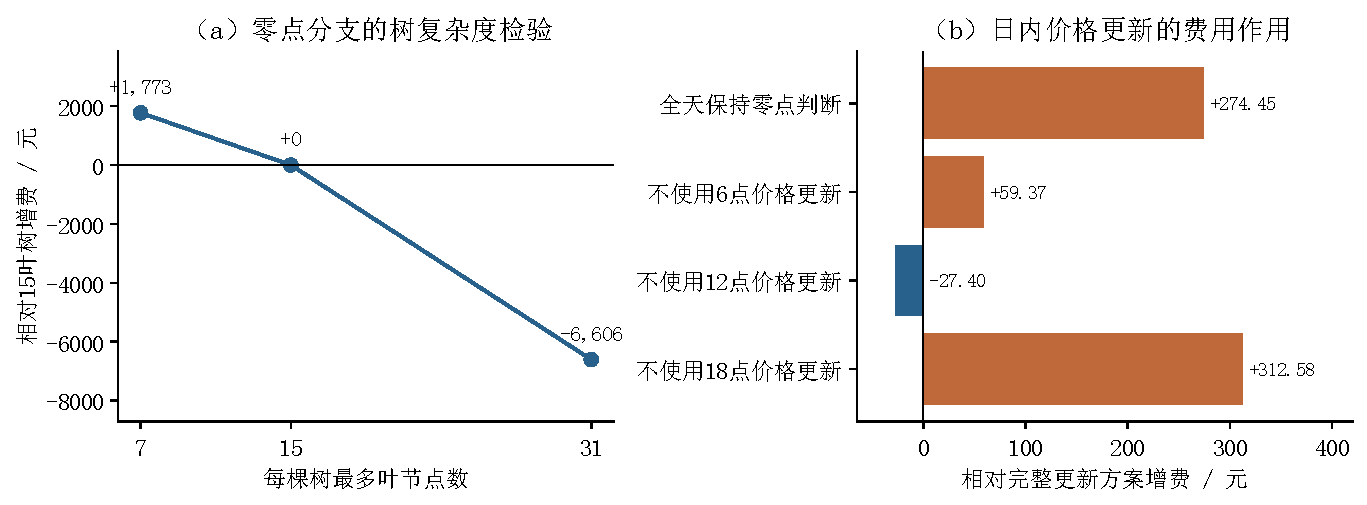
\includegraphics[width=.96\linewidth]{问题四模型检验.pdf}
\caption{树复杂度与日内价格更新的费用检验}
\label{fig:q4check}
\end{figure}

在实际价格最高的5\%区间内，问题四-2仍有46086.96~kWh紧急购电，问题四-3仍有14665.07~kWh。这说明储能受容量和放电功率限制，不能完全消除连续高价与供需偏差叠加的风险。进一步对期末库存按三档价格估值后，31叶树相对15叶树仍节省5890.24--6423.72元，说明它并非仅靠少留库存降低费用。

综上，波动电价下应先利用历史价格和当前可得信息判断未来价格，再通过线性规划统一安排普通购电与储能。问题四-2采用滚动提升树--零点线性规划模型，总费用为14248570.87元；问题四-3采用滚动岭回归--日内调整线性规划模型，总费用为13822901.35元。现有检验支持这两种模型在2025年数据范围内的选择，但参数比较仍基于同一年数据，结论不能直接推广到其他年份或其他微网。


\section{模型评价与推广}

\subsection{模型优点与创新}

\textbf{（1）四问共用一套可以核对的电量流骨架。}本文始终用十分钟电量连接负载、光伏、外网和电池，并统一处理90\%充电效率、90\%放电效率、储电上下限及功率限制。各问只在信息条件和费用规则发生变化时增加相应模块，避免同一物理过程被重复解释成不同含义。问题一的确定性调度由线性规划完成\cite{dantzig}，后续各问沿用同一基础关系，便于逐段复算。

\textbf{（2）把预测和高价缺口风险分开处理。}负载与光伏分别预测，使星期用电规律和近期光伏变化都能被解释\cite{hyndman}；误差准备则专门处理五倍紧急电价造成的损失不对称。候选比较显示，提升树即使改善部分预测误差，也没有超过带近期准备的完整方案。该设计说明模型追求的是最终运行费用和供电可靠性，而不是单一的拟合指标。

\textbf{（3）把日内信息的价值拆成两个可说明的部分。}问题三没有把197.28万元的总差额全部归功于新预报，而是先计算日内反馈与改单节省的175.51万元，再计算后发官方预报额外节省的21.78万元。这样可以直接回答题目关于日内预报是否值得引入的问题，也避免把权限变化误写成预测方法的贡献。

\textbf{（4）根据决策方式选择价格模型。}问题四没有机械地给两条分支使用同一种算法。零点分支采用提升树表达非线性关系\cite{friedman}；日内分支采用岭回归稳定处理高度相关的历史价格特征\cite{hoerl}。后者以极小费用差换取更少紧急购电和更清楚的系数含义，体现了经济性、风险和可解释性的综合选择。

\textbf{（5）结论能够追溯到实际运行过程。}本文使用SciPy和scikit-learn完成数值计算与候选预测\cite{virtanen,pedregosa}，线性规划由HiGHS求解\cite{huangfu}。全年费用均由保存的普通订单、紧急购电和储电轨迹重新计算，并逐段检查供需、库存、功率和结算关系。指定日期的图表进一步说明电池何时补缺、何时达到下限以及为什么仍会发生紧急购电，使模型结论既有总量证据，也有运行过程支撑。

\subsection{模型局限与改进方向}

首先，历史窗口、误差分位、日期衰减和价格模型参数主要在2025年数据内比较。现有结果能够说明本题数据范围内的取舍，但不能证明同一组参数在其他年份或其他地区仍然最优。若获得跨年数据，可按年份滚动回测，并在不同季节分别校准参数，以检验真正的跨年泛化能力。

其次，本文先预测负载、光伏和价格，再把预测结果送入优化。这样的分层结构容易解释，也便于定位误差来源，但没有同时描述三类不确定量可能共同出现的极端情景。后续可构造少量有现实含义的联合情景，比较连续阴天、高负载和高电价叠加时的计划，进一步控制尾部风险。

再次，题目没有提供电池老化费用、外送电价、网络损耗和可中断负载信息，因此本文未把这些因素写入目标函数。若用于真实微网，可增加循环寿命成本、需求响应和售电约束；末端库存的参考价值也应根据下一日市场规则重新估计，而不能直接视为可出售资产。

\subsection{模型推广性评估}

模型的核心输入只有分时负载、本地可再生能源、设备参数、交易价格和允许的决策时点。替换这些数据并重新校准预测与准备参数后，可用于社区、校园、工业园区及偏远地区的微网运行，也可扩展到多台储能、风光互补、充电站和可调负载。滚动求解方式允许系统随着新数据修正未来计划，适合部署在需要持续更新的能源管理平台中。

从社会应用看，该方法优先消纳本地光伏，并通过储能和合理购电减少高峰期对外网的额外压力，有助于提高可再生能源利用率、降低能源浪费，服务碳达峰和碳中和目标\cite{carbonplan,energyplan}。推广时还应把安全供电和居民基本用电放在成本优化之前，使节费收益建立在可靠、公平的能源服务之上。这样的应用方向既符合绿色发展和资源节约要求，也体现以人民为中心、共建共享的发展取向。

\newpage
\begin{thebibliography}{99}
\bibitem{dantzig} Dantzig G B. Linear Programming and Extensions[M]. Princeton: Princeton University Press, 1963.
\bibitem{hoerl} Hoerl A E, Kennard R W. Ridge regression: Biased estimation for nonorthogonal problems[J]. Technometrics, 1970, 12(1): 55--67.
\bibitem{friedman} Friedman J H. Greedy function approximation: A gradient boosting machine[J]. The Annals of Statistics, 2001, 29(5): 1189--1232.
\bibitem{huangfu} Huangfu Q, Hall J A J. Parallelizing the dual revised simplex method[J]. Mathematical Programming Computation, 2018, 10(1): 119--142.
\bibitem{hyndman} Hyndman R J, Athanasopoulos G. Forecasting: Principles and Practice[M]. 3rd ed. Melbourne: OTexts, 2021.
\bibitem{virtanen} Virtanen P, Gommers R, Oliphant T E, et al. SciPy 1.0: Fundamental algorithms for scientific computing in Python[J]. Nature Methods, 2020, 17: 261--272.
\bibitem{pedregosa} Pedregosa F, Varoquaux G, Gramfort A, et al. Scikit-learn: Machine learning in Python[J]. Journal of Machine Learning Research, 2011, 12: 2825--2830.
\bibitem{carbonplan} 国务院. 2030年前碳达峰行动方案[Z]. 2021.
\bibitem{energyplan} 国家发展改革委, 国家能源局. “十四五”现代能源体系规划[Z]. 2022.
\end{thebibliography}


\end{document}
